\documentclass[12pt,a4paper]{article}
\usepackage[T5]{fontenc}
\usepackage{indentfirst}
\usepackage[utf8]{inputenc}
\usepackage{lmodern} % <-- Gói này giúp font Computer Modern hỗ trợ tiếng Việt cực kỳ sắc nét
\usepackage[vietnamese]{babel}
\usepackage{amsmath,amssymb,amsfonts}
\newtheorem{definition}{Định nghĩa}[section]
\newtheorem{theorem}{Định lý}[section]
\usepackage{pgfkeys}

% Căn lề trang chuẩn báo cáo học thuật
\usepackage{geometry}
\geometry{a4paper, top=2.5cm, bottom=2.5cm, left=3cm, right=2.5cm}
% Thiết lập độ giãn dòng 1.25 giống ảnh mẫu
\usepackage{setspace}
\setstretch{1.25}
\usepackage{float}
\usepackage{booktabs}
% Định nghĩa bảng màu học thuật
\usepackage{xcolor}
\definecolor{titleblue}{RGB}{35, 75, 135} % Màu xanh chuẩn của các đầu mục
\definecolor{linkblue}{RGB}{0, 102, 204}

% Định dạng màu sắc và font chữ cho các cấp tiêu đề (Section, Subsection)
\usepackage{titlesec}
\titleformat{\section}{\normalfont\Large\bfseries\color{titleblue}}{\thesection.}{0.5em}{}
\titleformat{\subsection}{\normalfont\large\bfseries\color{titleblue}}{\thesubsection.}{0.5em}{}
\titleformat{\subsubsection}{\normalfont\large\bfseries\color{titleblue}}{\thesubsubsection.}{0.5em}{}

% Tối ưu khoảng cách giữa các mục trong danh sách bullet (itemize)
\usepackage{enumitem}
\setlist[itemize]{leftmargin=*, itemsep=0.4em, topsep=0.3em}

% code
\usepackage{xcolor}
\usepackage{listings}

\definecolor{codegreen}{RGB}{0,120,0}
\definecolor{codegray}{RGB}{110,110,110}
\definecolor{codeblue}{RGB}{0,0,180}
\definecolor{backcolour}{RGB}{248,248,248}
% Định nghĩa đúng 2 mã màu lấy từ ảnh mẫu
\definecolor{XanhTieuDe}{RGB}{0, 102, 34}    % Xanh lá đậm cho viền và tiêu đề
\definecolor{XanhNen}{RGB}{234, 245, 238}    % Xanh lá nhạt cho nền nội dung

\lstdefinestyle{MatlabStyle}{
    language=Matlab,
    backgroundcolor=\color{backcolour},
    basicstyle=\ttfamily\small,
    keywordstyle=\color{blue}\bfseries,
    commentstyle=\color{codegreen}\itshape,
    stringstyle=\color{red},
    numbers=left,
    numberstyle=\tiny\color{codegray},
    stepnumber=1,
    numbersep=10pt,
    frame=single,
    framesep=8pt,
    rulecolor=\color{gray},
    breaklines=true,
    breakatwhitespace=true,
    showstringspaces=false,
    tabsize=4,
    columns=fullflexible,
    keepspaces=true
}


% Cấu hình siêu liên kết mục lục
\usepackage{hyperref}
\usepackage{xcolor}
\hypersetup{
    colorlinks=true,
    linkcolor=titleblue,
    filecolor=magenta,      
    urlcolor=linkblue,
    % Các phương trình dùng \tag{} thủ công nên không tăng bộ đếm equation;
    % hypertexnames=false buộc hyperref sinh tên đích duy nhất cho từng liên kết.
    hypertexnames=false,
}

\usepackage[most]{tcolorbox}
\newtcolorbox{baitapbox}[1]{
  colback=blue!5, colframe=blue!60!black, coltitle=white, 
  fonttitle=\bfseries, enhanced, title=#1,
}

\newtcolorbox{vidu}[1]{
  colback=XanhNen, 
  colframe=XanhTieuDe, 
  coltitle=white,
  fonttitle=\bfseries, 
  title=#1
}

\newtcolorbox{bode}[1]{ 
	enhanced, 
	colback=red!5!white, 
	colframe=red, 
	boxrule=0.5pt,
	arc=2mm,
	title={#1}, 
	fonttitle=\bfseries, 
	colbacktitle=red,
	attach boxed title to top left={xshift=5mm, yshift=-2.5mm}, 
	boxed title style={arc=3mm,, size=small}
}

\title{\color{titleblue}\textbf{PHƯƠNG PHÁP ĐA BƯỚC TUYẾN TÍNH}\\[0.4em]
\large \textit{\color{black}Sai số, tính nhất quán, tính 0-ổn định và sự hội tụ}\\[0.2em]
\large \textit{\color{black}cùng định lý tương đương Dahlquist}\\[0.8em]
\normalsize \color{black}Báo cáo môn Giải tích số cho Phương trình vi phân\\[0.2em]
\normalsize \color{black}Trường Đại học Khoa học Tự nhiên, ĐHQG-HCM}
% Điền tên nhóm thực hiện vào đây trước khi nộp / công bố.
\author{}
\date{\today}

\begin{document}

\maketitle
\tableofcontents
\newpage

% ==========================================
\newpage
\section*{Lời cảm ơn}

Trước hết, nhóm chúng em xin bày tỏ lòng biết ơn chân thành đến Trường Đại học Khoa học Tự nhiên, Đại học Quốc gia Thành phố Hồ Chí Minh đã tạo điều kiện thuận lợi về môi trường học tập, cơ sở vật chất và chương trình đào tạo để chúng em có cơ hội tiếp cận, nghiên cứu môn học \textit{Giải tích số cho Phương trình vi phân}.

Đặc biệt, chúng em xin gửi lời cảm ơn sâu sắc đến Thầy TS. Nguyễn Đăng Khoa, giảng viên trực tiếp phụ trách môn học. Trong suốt quá trình học tập và thực hiện báo cáo, thầy đã tận tình truyền đạt kiến thức chuyên môn, định hướng phương pháp nghiên cứu, đồng thời luôn sẵn sàng giải đáp những thắc mắc và góp ý quý báu. Những hướng dẫn của thầy là nguồn động viên và là nền tảng quan trọng giúp chúng em hoàn thành báo cáo này.

Bên cạnh đó, chúng em cũng xin trân trọng cảm ơn các tác giả của những giáo trình, sách chuyên khảo, bài báo khoa học và các tài liệu tham khảo đã được sử dụng trong quá trình thực hiện báo cáo. Những tài liệu này đã cung cấp cơ sở lý thuyết và nguồn tư liệu quý giá, giúp chúng em có cái nhìn đầy đủ và hệ thống hơn về nội dung nghiên cứu.

Mặc dù đã cố gắng hoàn thành báo cáo một cách tốt nhất, do kiến thức và kinh nghiệm còn hạn chế nên báo cáo khó tránh khỏi những thiếu sót. Chúng em rất mong nhận được những ý kiến đóng góp và nhận xét từ quý thầy để tiếp tục hoàn thiện kiến thức và nâng cao kỹ năng nghiên cứu.

\vspace{0.5cm}
\begin{flushright}
\textbf{Nhóm thực hiện}
\end{flushright}

\newpage
\section*{Lời nói đầu}
Phương trình vi phân thường là công cụ nền tảng mô tả cho vô số hiện tượng trong khoa học tự nhiên, kỹ thuật và kinh tế: từ chuyển động cơ học, phản ứng hoá học, mạch điện, đến các mô hình quần thể sinh học và tài chính. Tuy nhiên, phần lớn các bài toán giá trị đầu xuất hiện trong thực tế không có nghiệm hiển, buộc ta phải tìm đến các phương pháp số để xấp xỉ nghiệm.

Trong số các lớp phương pháp số giải bài toán giá trị đầu:
\[
    y'(t) = f(t,y(t)), \qquad y(t_0) = y_0,
\]

Phương pháp đa bước tuyến tính - LMM là một lớp phương pháp quan trọng nhờ khả năng khai thác thông tin từ nhiều bước tính trước để nâng cao hiệu quả tính toán. Lý thuyết của LMM cũng là một trong những nền tảng của giải tích số hiện đại, đặc biệt thông qua các kết quả về tính nhất quán, tính ổn định và tính hội tụ.

Năm 1956, Germund Dahlquist đã thiết lập một kết quả cơ bản trong lý thuyết phương pháp đa bước tuyến tính, thường được gọi là định lý tương đương Dahlquist. Định lý phát biểu rằng: \textit{``Một phương pháp đa bước tuyến tính hội tụ khi và chỉ khi nó nhất quán và $0$-ổn định''}.

Định lý này chỉ ra rằng tính hội tụ của một phương pháp đa bước tuyến tính có thể được đặc trưng hoàn toàn bởi hai tính chất cơ bản là tính nhất quán và $0$-ổn định. Vì hai tính chất này có thể được kiểm tra trực tiếp từ cấu trúc của phương pháp, kết quả trên đóng vai trò quan trọng trong việc phân tích và xây dựng các phương pháp số.

Báo cáo này trình bày một cách hệ thống các khái niệm về tính nhất quán, $0$-ổn định và tính hội tụ của phương pháp đa bước tuyến tính, đồng thời giới thiệu nội dung và ý nghĩa của định lý tương đương Dahlquist. Bên cạnh phần lý thuyết, báo cáo cũng trình bày các ví dụ minh họa cho họ phương pháp đa bước tuyến tính phổ biến Backward Differentiation Formulas (BDF).

Nhóm chúng em xin chân thành cảm ơn thầy TS.Nguyễn Đăng Khoa đã hướng dẫn và góp ý trong suốt quá trình thực hiện báo cáo này.

\newpage
\section*{Mã nguồn đi kèm}
Toàn bộ kết quả số trong báo cáo này được sinh lại bằng mã nguồn công khai đi kèm.
Thư viện Python \texttt{lmm} suy ra trực tiếp từ bộ hệ số $(\alpha_j,\beta_j)$ của một
phương pháp: bậc chính xác, hằng số sai số, điều kiện nghiệm, tính 0-ổn định và miền
ổn định tuyệt đối; các script trong \texttt{code/experiments/} tái tạo mọi bảng số và
hình vẽ, còn bộ kiểm thử trong \texttt{code/tests/} kiểm chứng bằng số các phát biểu
lý thuyết được chứng minh ở các chương sau (kể cả rào cản Dahlquist và giới hạn
$k \leq 6$ của họ BDF).

\begin{center}
\url{https://github.com/tu-h-nguyn/Stability-Consistency-and-Convergence-of-Linear-Multistep-Methods}
\end{center}

\newpage
\section{Chương 1. Mở đầu và một số kiến thức chuẩn bị}

\subsection{Một số kiến thức chuẩn bị}
    Trước khi đi sâu vào việc thiết lập công thức và khảo sát sự hội tụ của phương pháp đa bước tuyến tính, ta cần chuẩn bị một số công cụ giải tích và đại số nền tảng. Cụ thể, \textit{khai triển Taylor} đóng vai trò là công cụ chủ chốt để xây dựng công thức xấp xỉ đạo hàm và đánh giá sai số chặt cụt; \textit{định lý tồn tại duy nhất Picard–Lindelöf} bảo đảm tính đặt chỉnh của bài toán giá trị đầu; và lý thuyết \textit{phương trình sai phân tuyến tính hệ số hằng cùng đa thức đặc trưng} là cơ sở để phân tích sai số và tính ổn định số của phương pháp số.
    
\subsubsection{Khai triển Taylor phần dư Lagrange}
Khai triển Taylor là công cụ toán học chủ chốt dùng để thiết lập các phương trình xấp xỉ đạo hàm và đánh giá sai số chặt cụt cục bộ (Local Truncation Error) của các phương pháp số.
\begin{baitapbox}{Công thức Taylor với phần dư dạng Lagrange}
    Giả sử hàm số $y(t)$ thuộc lớp khả vi liên tục $C^{m+1}([t_0, T])$. Khi đó, với mọi $t, t + h \in [t_0, T]$, giá trị của hàm tại điểm kề tiếp có thể được biểu diễn dưới dạng:
    \begin{equation}
        y(t + h) = y(t) + h y'(t) + \frac{h^2}{2!} y''(t) + \dots + \frac{h^m}{m!} y^{(m)}(t) + R_m(t) \tag{1.1} \label{eq:1.1}
    \end{equation}
    \noindent trong đó $R_m(t)$ là số dư bậc $m$, được xác định bởi:
    \[
        R_m(t) = \frac{h^{m+1}}{(m+1)!} y^{(m+1)}(\xi), \qquad \xi \in (\min(t, t+h), \max(t, t+h)).
    \]

\end{baitapbox}
\textbf{Ý nghĩa trong phương pháp đa bước:} Khi khai triển giá trị $y(t_n + jh)$ và đạo hàm $y'(t_n + jh) = f(t_{n+j}, y_{n+j})$ xung quanh điểm nút $t_n$, các tổ hợp tuyến tính của chúng cho phép triệt tiêu các bậc đạo hàm thấp của $h$, từ đó xây dựng được công thức đa bước đạt bậc chính xác $p$ mong muốn (tức phần dư $R_p \sim \mathcal{O}(h^{p+1})$).\\



Tính đặt chỉnh (well-posedness) của bài toán giá trị đầu (IVP) là tiền đề bắt buộc trước khi áp dụng bất kỳ thuật toán xấp xỉ số nào. Nếu phương trình vi phân ban đầu không có nghiệm duy nhất hoặc nghiệm phụ thuộc không liên tục vào dữ liệu ban đầu, mọi xấp xỉ số đều mất ý nghĩa thực tiễn.

\subsubsection{Tính liên tục Lipschitz}

\begin{baitapbox}{Điều kiện Lipschitz}
Hàm $f(t, y)$ định nghĩa trên miền $D \subset \mathbb{R} \times \mathbb{R}^d$ được gọi là thỏa mãn điều kiện Lipschitz theo biến $y$ trên $D$ với hằng số $L > 0$ nếu:
\[
    \|f(t, u) - f(t, v)\| \le L\|u - v|, \qquad \forall (t, u), (t, v) \in D.
\]
\end{baitapbox}

\subsubsection{Sự tồn tại nghiệm và định lý Picard--Lindelöf}

\begin{baitapbox}{Định lý Picard - Lindelöf}
    \begin{enumerate}
        \item Nếu $f$ liên tục trên miền hình chữ nhật:
        \[
        R = \{(t,y): t_0 \le t \le T_{max}\}
        \]
        \item Hàm số $f$ bị chặn trên miền hình chữ nhật:
        \[
        M_0 =max\{|f(t;y)|:(t;y) \in R\}
        \]
        và hơn nữa $M_0(T_{max} - t_0) \le y_M$
        \item Nếu $f$ liên tục theo $t$ và Lipschitz theo biến $y$, tức tồn tại $L > 0$ sao cho
        \[
        \|f(t, u) - f(t, v)\| \le L\|u - v\|, \qquad \forall t \in [t_0, T], \quad \forall u, v \in \mathbb{R}^d,
        \]
    \end{enumerate}
   
    Nếu $f$ thỏa mãn các điều kiện trên thì tồn tại $\epsilon > 0$ sao cho bài bài toán
    \[
    y'(t) = f(t, y(t)), \qquad t \in [t_0, T_{max}], \qquad y(t_0) = y_0
    \]
    có duy nhất nghiệm $y(t)$ trong đoạn $[t_0-\epsilon;t_0+\epsilon]$
\end{baitapbox}

\subsubsection{Phương trình sai phân tuyến tính hệ số hằng và đa thức đặc trưng}

Trong lý thuyết hội tụ của phương pháp đa bước, hằng số Lipschitz $L$ đóng vai trò quyết định trong việc thiết lập giới hạn lan truyền của sai số toàn cục thông qua Bổ đề Gronwall rời rạc.

Khi khảo sát hành vi tiệm cận của phương pháp đa bước lúc bước nhảy $h \to 0$, bài toán được quy về việc phân tích nghiệm của một phương trình sai phân thuần nhất tuyến tính.
\begin{baitapbox}{Phương trình sai phân tuyến tính và đa thức đặc trưng}
    Xét phương trình sai phân tuyến tính cấp $k$ với hệ số hằng:
\begin{equation}
    \alpha_k y_{n+k} + \alpha_{k-1} y_{n+k-1} + \dots + \alpha_0 y_n = 0, \qquad (\alpha_k \neq 0, \, \alpha_0 \neq 0). \tag{1.2} \label{eq:1.2}
\end{equation}
\noindent Để giải phương trình \eqref{eq:1.2}, ta tìm nghiệm dưới dạng $y_n = \zeta^n$ ($\zeta \in \mathbb{C}$, $\zeta \neq 0$). Thay vào phương trình, ta thu được \textit{đa thức đặc trưng}:
\begin{equation}
    \rho(\zeta) = \alpha_k \zeta^k + \alpha_{k-1} \zeta^{k-1} + \dots + \alpha_0 = \sum_{j=0}^k \alpha_j \zeta^j = 0. \tag{1.3} \label{eq:1.3}
\end{equation}

\noindent Cấu trúc nghiệm tổng quát của phương trình sai phân \eqref{eq:1.2} hoàn toàn phụ thuộc vào nghiệm của phương trình đại số \eqref{eq:1.3}:
\begin{itemize}
    \item Nếu $\zeta_i$ là một nghiệm đơn của $\rho(\zeta) = 0$, nó đóng góp một nghiệm riêng dạng $y_n^{(i)} = C_i \zeta_i^n$.
    \item Nếu $\zeta_j$ là một nghiệm bội bậc $m_j$ của $\rho(\zeta) = 0$, nó đóng góp $m_j$ nghiệm độc lập tuyến tính dạng:
    \[
        y_n^{(j, 0)} = \zeta_j^n, \quad y_n^{(j, 1)} = n \zeta_j^n, \quad \dots, \quad y_n^{(j, m_j-1)} = n^{m_j-1} \zeta_j^n.
    \]
\end{itemize}
\end{baitapbox}

\noindent \textbf{Hệ quả đối với tính ổn định:} Dãy nghiệm xấp xỉ $\{Y_n\}$ bị chặn (không bùng nổ vô hạn khi $n \to \infty$) khi và chỉ khi mọi nghiệm của phương trình đặc trưng thỏa mãn $|\zeta_i| \le 1$, và nếu có nghiệm nằm trực tiếp trên đường tròn đơn vị ($|\zeta_i| = 1$) thì nghiệm đó buộc phải là nghiệm đơn. Đây chính là nền tảng toán học của \textit{Điều kiện nghiệm Dahlquist (Root Condition)}.

%\subsubsection{Tính nhất quán, ổn định và sự hội tụ của một phương pháp số}
%Trước khi đi vào phân tích và tìm các điều kiện, hệ điều kiện để phương pháp đa bước tuyến tính nhất quán, ổn định, hội tụ. Ta cùng nhắc lại các định nghĩa tổng quát của tính \textit{nhất quán}, \textit{ổn định} và \textit{hội tụ}.
\subsubsection{Phép nội suy Lagrange}
\begin{baitapbox}{Đa thức nội suy Lagrange}
    Cho $n+1$ điểm dữ liệu $(x_0, y_0), (x_1, y_1), \dots, (x_n, y_n)$. Đa thức nội suy $P(x)$ bậc không vượt quá $n$ có dạng tổng quát:
\[
P(x) = \sum_{i=0}^{n} y_i L_i(x)
\]
Trong đó, $L_i(x)$ là các đa thức cơ sở Lagrange được tính theo công thức:
\[
L_i(x) = \prod_{j=0\\ j \neq i}^{n} \frac{x - x_j}{x_i - x_j} = \frac{(x-x_0)\dots(x-x_{i-1})(x-x_{i+1})\dots(x-x_n)}{(x_i-x_0)\dots(x_i-x_{i-1})(x_i-x_{i+1})\dots(x_i-x_n)}
\]
\end{baitapbox}

\subsection{Bài toán giá trị đầu (IVP) và sự cần thiết của phương pháp số}

Xét bài toán giá trị ban đầu đối với phương trình vi phân thường
\begin{equation}
    y'(t) = f(t, y(t)), \qquad t \in [t_0, T_{max}], \qquad y(t_0) = y_0, \tag{1.1} \label{eq:1.1}
\end{equation}
\noindent trong đó $y(t) \in \mathbb{R}^d$, $f : [t_0, T] \times \mathbb{R}^d \to \mathbb{R}^d$ là hàm đã cho.Ta giả sử $f$ liên tục theo $t$ và Lipschitz theo biến $y$, tức tồn tại $L > 0$ sao cho
        \[
        \|f(t, u) - f(t, v)\| \le L\|u - v\|, \qquad \forall t \in [t_0, T], \quad \forall u, v \in \mathbb{R}^d,
        \]

Hiển nhiên theo định lý Picard thì \eqref{eq:1.1} có duy nhất nghiệm $y(t)$ trên đoạn $[t_0 - \epsilon;t_o + \epsilon]$. Trong báo cáo này ta giả sử nghiệm đủ trơn để các khai triển Taylor cần thiết đều hợp lệ.

Để tính nghiệm số, ta chia đoạn $[t_0, T]$ thành $N$ đoạn con bằng nhau:
\[
    h = \frac{T - t_0}{N}, \qquad t_n = t_0 + nh, \qquad n = 0, 1, \dots, N.
\]

Ta cần xây dựng dãy $Y_n$ sao cho
\[
    Y_n \approx y(t_n).
\]

Sai số tại nút $t_n$ thường được gọi là sai số toàn cục:
\[
    e_n = y(t_n) - Y_n.
\]

Mục tiêu cuối cùng là khi cho bước lưới tiến về 0 $h \to 0$ thì ta đi tìm các điều kiện, hệ điều kiện để $\max \|e_n\| \to 0$.\\

% Trong thế giới thực, các định lý tự nhiên thường được biểu diễn dưới dạng mối liên hệ giữa \textbf{trạng thái hiện tại} của hệ thống và \textbf{tốc độ thay đổi} của nó. Do đó, IVP đóng vai trò là “ngôn ngữ cơ bản” để mô hình hóa sự tiến hóa động theo thời gian:

% \begin{itemize}[leftmargin=*]
%     \item \textbf{Cơ học \& Kỹ thuật hàng không:} Định luật II Newton $m\mathbf{a} = \mathbf{F}(t, \mathbf{x}, \mathbf{v})$ được viết dưới dạng IVP để dự đoán quỹ đạo bay của tên lửa, vệ tinh hoặc tàu vũ trụ dựa trên vị trí và vận tốc lúc phóng ($t=0$).
%     \item \textbf{Kỹ thuật điện \& Điện tử:} Phân tích quá độ trong các mạch điện RLC, hệ thống điều khiển tự động nơi điện áp và dòng điện phụ thuộc vào các điều kiện ban đầu của tụ điện và cuộn cảm.
%     \item \textbf{Sinh học \& Dịch tễ học:} Các mô hình truyền nhiễm (như mô hình SIR/SEIR) dự báo sự lây lan của dịch bệnh từ một số lượng ca nhiễm khởi phát ban đầu $I(0) = I_0$.
%     \item \textbf{Kỹ thuật Hóa học:} Mô phỏng động học phản ứng nồng độ các chất trong lò phản ứng liên tục theo thời gian.
% \end{itemize}    

% Dù việc tìm nghiệm giải tích (nghiệm chính xác dưới dạng công thức toán học tường minh $y(t)$) luôn là lý tưởng, nhưng trong thực tế kỹ thuật, ta \textbf{bắt buộc phải dùng phương pháp số} vì các lý do toán học và thực tiễn sau:

% \begin{itemize}[leftmargin=*]
%     \item \textbf{Sự thống trị của tính phi tuyến (Nonlinearity):}
%     Chỉ một lớp rất nhỏ các phương trình vi phân (như phương trình tuyến tính, phương trình biến số phân ly, Bernoulli, Euler...) mới có nghiệm giải tích. Hầu hết các bài toán thực tế chứa các phần tử phi tuyến phức tạp (ví dụ: lực cản không khí tỷ lệ với $v^2$, dao động con lắc lớn $\sin\theta$). Các phương trình phi tuyến này không tồn tại nghiệm biểu diễn qua các hàm sơ cấp.
    
%     \item \textbf{Quy mô hệ phương trình lớn (Curse of Dimensionality):}
%     Khi rời rạc hóa các phương trình vi phân riêng phần (PDEs) theo phương pháp đường (Method of Lines) — ví dụ như phương trình Navier-Stokes trong động lực học lưu chất (CFD) hay truyền nhiệt — ta nhận được hệ IVP gồm hàng nghìn đến hàng triệu phương trình ODE liên kết với nhau ($d = 10^3 \sim 10^6$). Việc giải tích cho các hệ này là bất khả thi.

%     \item \textbf{Dữ liệu thực nghiệm dạng bảng (Empirical Data):}
%     Trong nhiều hệ thống kỹ thuật, hàm $f(t, y)$ không được cho bởi một công thức toán học khép kín mà được thu thập qua thực nghiệm, bảng tra cứu (lookup tables) hoặc các cảm biến đo đạc thời gian thực theo từng bước rời rạc. Phương pháp giải tích không thể áp dụng cho các hàm không tường minh này.

%     \item \textbf{Tính hiệu quả và khả năng kiểm soát sai số:}
%     Các phương pháp số (như Euler, Runge-Kutta RK4, Adams-Bashforth) cho phép thay thế việc giải phương trình vi phân liên tục bằng một chuỗi các phép tính đại số lặp trên lưới thời gian rời rạc $t_n = t_0 + nh$. Ngay cả khi bài toán có nghiệm giải tích (thường chứa các tích phân không thể tính đúng hoặc chuỗi vô hạn), phương pháp số cung cấp giá trị xấp xỉ $y_n \approx y(t_n)$ nhanh hơn, dễ lập trình hơn trên máy tính và có thể kiểm soát được sai số làm tròn/sai số phương pháp.
% \end{itemize}



\subsection{Tổng quan về phương pháp số một bước và đa bước}

Trong giải tích số, các phương pháp xấp xỉ nghiệm của bài toán giá trị đầu (IVP) \eqref{eq:1.1} được chia thành hai họ chính dựa trên số lượng mốc thời gian quá khứ được sử dụng để tính toán trạng thái tiếp theo.

\subsubsection{Phương pháp một bước}
Phương pháp một bước là lớp phương pháp mà để tính giá trị xấp xỉ $y_{n+1} \approx Y(t_{n+1})$ tại mốc thời gian mới, thuật toán \textbf{chỉ sử dụng thông tin từ mốc thời gian liền trước đó} là $(t_n, y_n)$. Công thức tổng quát của họ phương pháp này có dạng:
\begin{equation}
    Y_{n+1} = Y_n + h \Phi(t_n, y_n, h), \tag{1.6}
\end{equation}
\noindent trong đó $\Phi$ được gọi là hàm gia số, đại diện cho độ dốc trung bình trên đoạn $[t_n, t_{n+1}]$.

\begin{itemize}[label=\null]
    \item \textbf{Đại diện tiêu biểu:} Phương pháp Euler (bậc 1) và họ phương pháp Runge--Kutta (như RK4 bậc 4).
    \item \textbf{Ưu điểm:} Tính tự khởi động, do chỉ phụ thuộc vào $y_n$, phương pháp có thể bắt đầu tính ngay từ điều kiện ban đầu $y_0$. Ngoài ra, việc thay đổi bước lưới $h$ trong quá trình tính toán diễn ra rất linh hoạt và dễ dàng.
    \item \textbf{Nhược điểm:} Để đạt được bậc chính xác cao $p$, phương pháp Runge--Kutta đòi hỏi phải đánh giá hàm đạo hàm $f(t, y)$ nhiều lần tại các điểm trung gian bên trong đoạn $[t_n, t_{n+1}]$ (ví dụ: RK4 cần $4$ lần tính hàm $f$ cho mỗi bước lưới). Đối với các bài toán có quy mô lớn hoặc hàm $f$ phức tạp, khối lượng tính toán này là một gánh nặng đáng kể.
\end{itemize}

\subsubsection{Phương pháp đa bước tuyến tính}
Khác với phương pháp một bước, phương pháp đa bước tận dụng quan điểm rằng các giá trị xấp xỉ ở những bước trước đó $(t_{n-1}, y_{n-1}), (t_{n-2}, y_{n-2}), \dots$ đã mang sẵn thông tin lịch sử về quỹ đạo của nghiệm. Do đó, thay vì bỏ đi và tính lại từ đầu, ta có thể tái sử dụng chúng.

Một phương pháp đa bước tuyến tính $k$-bước có dạng tổng quát:
\begin{equation}
    \sum_{j=0}^{k} \alpha_j y_{n+j} = h \sum_{j=0}^{k} \beta_j f(t_{n+j}, y_{n+j}), \qquad \alpha_k \neq 0, \quad |\alpha_0| + |\beta_0| > 0. \tag{1.7}
\end{equation}

\textbf{Ưu thế vượt trội về khối lượng tính toán:} 
Trong công thức (1.7), để bước tới điểm mới $y_{n+k}$, tất cả các giá trị hàm trong quá khứ $f(t_{n+j}, y_{n+j})$ với $j = 0, 1, \dots, k-1$ đều đã được tính và lưu trong bộ nhớ từ các bước lặp trước. 
\begin{itemize}[label=\null]
    \item Đối với phương pháp hiện ($\beta_k = 0$), ta chỉ cần đúng \textbf{1 lần} đánh giá hàm $f$ mới tại mỗi bước tính, bất kể bậc chính xác $p$ cao đến đâu.
    \item Đối với phương pháp ẩn ($\beta_k \neq 0$), khi kết hợp dưới dạng cặp Dự đoán -- Hiệu chỉnh, số lượng đánh giá hàm $f$ cho mỗi bước cũng chỉ từ $1$ đến $2$ lần.
\end{itemize}

Nhờ sự tiết kiệm tối đa khối lượng tính hàm $f(t, y)$, phương pháp đa bước tuyến tính trở thành công cụ lý tưởng cho các hệ vi phân lớn trong thực tiễn kỹ thuật. Tuy nhiên, đánh đổi lại, phương pháp này \textit{không có khả năng tự khởi động} (bắt buộc phải dùng phương pháp một bước để tạo mồi $k$ giá trị đầu) và việc quản lý tính ổn định số trở nên phức tạp hơn rất nhiều.


\subsection{Mục tiêu và phạm vi của báo cáo}

Báo cáo này tập trung đi sâu vào khung lý thuyết, phân tích cấu trúc sai số và khảo sát sự hội tụ của các phương pháp đa bước tuyến tính trong giải tích số. Cụ thể, báo cáo xoay quanh việc chứng minh và làm sáng tỏ định lý tương đương giữa hội tụ và ``nhất quán $+$ ổn định (0-ổn định)'', áp dụng cho một số công thức Adams và đặc biệt là họ công thức vi phân lùi BDF (Backward Differentiation Formulas) cơ bản.

Nội dung và mục tiêu trọng tâm của báo cáo được cụ thể hóa qua $5$ nội dung sau:
\begin{enumerate}
    \item Trình bày định nghĩa sai số chặt cụt, tính nhất quán và ổn định (0-ổn định) của phương pháp đa bước.
    \item Xây dựng đa thức đặc trưng và kiểm tra điều kiện nghiệm cho một số phương pháp cụ thể.
    \item Giới thiệu và khảo sát các công thức BDF bậc thấp; xác định khi nào các công thức này nhất quán và 0-ổn định.
    \item Trình bày chứng minh hoặc phác thảo chứng minh định lý hội tụ chính.
    \item Thực hiện ví dụ số minh họa một phương pháp nhất quán nhưng không hội tụ khi không thoả điều kiện ổn định.
\end{enumerate}



%\begin{itemize}
%    \item Ý tưởng cơ bản của phương pháp một bước (chỉ dùng thông tin tại $t_n$ để tính $t_{n+1}$).
%    \item Ý tưởng và ưu thế về khối lượng tính toán của phương pháp đa bước tuyến tính (LMM) sử dụng thông tin từ nhiều mốc thời gian quá khứ.
%\end{itemize}


% ==========================================
\newpage 

\section{Chương 2. Phương pháp đa bước tuyến tính, các loại sai số và tính nhất quán, ổn định, hội tụ}

\subsection{Lưới thời gian, phân loại phương pháp và sai số}
%\begin{itemize}
%    \item Định nghĩa lưới thời gian đều với bước nhảy $h$: $t_n = t_0 + nh$.
%    \item Công thức tổng quát của phương pháp đa bước tuyến tính $k$-bước:
%    \[
%        \sum_{j=0}^{k} \alpha_j y_{n+j} = h \sum_{j=0}^{k} \beta_j f(t_{n+j}, y_{n+j}), \quad \alpha_k \neq 0, \quad |\alpha_0| + |\beta_0| > 0.
%    \]
%\end{itemize}

Để tìm nghiệm xấp xỉ của bài toán giá trị đầu (IVP) trên đoạn $[t_0, T]$, bước đầu tiên là rời rạc hóa miền thời gian liên tục thành một tập hợp hữu hạn các điểm nút.
\subsubsection{Lưới thời gian và công thức tổng quát của phương pháp đa bước}
Ta chia đoạn $[t_0, T]$ thành $N$ đoạn con bằng nhau bởi một \textit{lưới thời gian đều} với bước nhảy $h > 0$:
\begin{equation}
    h = \frac{T - t_0}{N}, \qquad t_n = t_0 + nh, \qquad n = 0, 1, \dots, N. \tag{2.1} \label{eq:2.1}
\end{equation}
\noindent Tại mỗi nút $t_n$, ký hiệu $y(t_n)$ là giá trị nghiệm chính xác (nghiệm giải tích) và $Y_n \approx y(t_n)$ là giá trị nghiệm số xấp xỉ cần tìm. Đồng thời, để viết gọn biểu thức, ta ký hiệu $f_n = f(t_n, y_n)$. 
%Ta bắt đầu từ bài toán (1.1), lấy tích phân hai vế từ $t_n$ đến $t_{n+1}$ ta được:
%\[
%\displaystyle \int_{t_n}^{t_{n+1}} y'(t)dt = \displaystyle \int_{t_n}^{t_{n+1}}f(y;y(t))dt
%\]
%Theo định lý cơ bản của giải tích ra được:
%\[
%y_{n+1}  = y_n +\displaystyle \int_{t_n}^{t_{n+1}}f(y;y(t))dt
%\]
%Tiếp theo ta chuẩn hóa các biến, đặt:
%\[
%t = t_n + sh \qquad 0 \le s\le1 
%\]
%Khi đó:
%\[
%dt = hds
%\]
%Vậy tích phân ở trên trở thành:
%\[
%y_{n+1} = y_n + \displaystyle h\int_{0}^{1}f(t_n + sh))ds
%\]
%Mặt khác, ta dùng nội suy Lagrange cho $f(t_n + sh)$ thì được:
%\[
%f(t_n + sh) \approx P(s) = \displaystyle \sum_{j=0}^{k-1}L_j(s) f_{n-j}
%\]
%Trong đó:
%\[
%L_j(s) = \displaystyle \prod_{m=0\\ m \ne j}^{k-1} \frac{s+m}{m-j}
%\]
%Thay vào tích phân ta được:
%\[
%y_{n+1} = y_n + h \displaystyle h\int_{0}^{1}P(s)ds = y_n + \displaystyle h\int_{0}^{1}\displaystyle %\sum_{j=0}^{k-1}L_j(s) f_{n-j}ds
%\]
%Do tích phân trên là tuyến tính nên:
%\[
%y_{n+1} = y_n + \displaystyle h\sum_{j=0}^{k-1} f_{n-j} \ \displaystyle h\int_{0}^{1}L_j(s)ds
%\]







Một phương pháp đa bước tuyến tính là một công thức sai phân liên hệ trạng thái mới $Y_{n}$ với các trạng thái trong quá khứ thông qua một tổ hợp tuyến tính giữa các giá trị nghiệm và các đạo hàm tương ứng:
\begin{equation}
    \sum_{j=0}^{k} \alpha_j Y_{n+j} = h \sum_{j=0}^{k} \beta_j f(t_{n+j}, Y_{n+j}), \tag{2.2} \label{eq:2.2}
\end{equation}
hoặc viết dưới dạng khai triển tường minh hơn:
\[
    \alpha_k Y_{n+k} + \alpha_{k-1} Y_{n+k-1} + \dots + \alpha_0 Y_n = h \left[ \beta_k f_{n+k} + \beta_{k-1} f_{n+k-1} + \dots + \beta_0 f_n \right].
\]

\begin{baitapbox}{Phương pháp đa bước tuyến tính $k$-bước}
    Một phương pháp đa bước tuyến tính được gọi là $k-$bước khi ít nhất một trong hai hệ số $\alpha_0$ hoặc $\beta_0$ là khác không. Điều này tương đương với:
    \[
    \sum_{j=0}^{k} \alpha_j Y_{n+j} = h \sum_{j=0}^{k} \beta_j f(t_{n+j}, Y_{n+j}) \qquad |\alpha_0| + |\beta_0| > 0
    \]
\end{baitapbox}

\vspace{0.5em}

%\noindent \textbf{Tư duy cấu trúc và điều kiện đặt chỉnh của công thức (2.2):}
%\begin{itemize}
%    \item \textbf{Hệ số chuẩn hóa ($\alpha_k \neq 0$):} Viết phương trình để giải tìm trạng thái mới nhất $y_{n+k}$, do đó hệ số đi kèm với nó bắt buộc phải khác không. Thông thường trong thực hành, ta chuẩn hóa $\alpha_k = 1$.
%    \item \textbf{Độ rộng bước thực sự ($|\alpha_0| + |\beta_0| > 0$):} Điều kiện này bảo đảm rằng mốc thời gian xa nhất trong quá khứ là $t_n$ thực sự tham gia vào công thức. Nếu cả $\alpha_0 = 0$ và $\beta_0 = 0$, công thức tự bị suy biến thành phương pháp $(k-1)$-bước.
%    \item \textbf{Tính tuyến tính:} Công thức được gọi là \textit{tuyến tính} vì nó chỉ là tổ hợp bậc nhất của các $y_{n+j}$ và $f_{n+j}$. Tuy nhiên, bản thân phương trình vi phân $f(t, y)$ hoàn toàn có thể phi tuyến phức tạp theo biến $y$.
%\end{itemize}

\subsubsection{Xây dựng đa thức đặc trưng thứ nhất và thứ hai}

Như đã khảo sát sơ bộ ở phần lý thuyết phương trình sai phân tuyến tính, cấu trúc nghiệm của một dãy truy hồi hệ số hằng được quyết định hoàn toàn bởi các nghiệm của đa thức đại số tương ứng. Đối với phương pháp đa bước tuyến tính tổng quát $k$-bước:
\begin{equation}
    \sum_{j=0}^{k} \alpha_j y_{n+j} = h \sum_{j=0}^{k} \beta_j f(t_{n+j}, y_{n+j}), \tag{2.3} \label{eq:2.3}
\end{equation}
ta có hai tập hợp hệ số độc lập là $\{\alpha_j\}_{j=0}^k$ và $\{\beta_j\}_{j=0}^k$. Để thuận tiện cho việc phân tích độ ổn định và sai số bằng các công cụ giải tích phức, người ta ánh xạ hai bộ hệ số này thành hai đa thức biến phức $\zeta$.

\vspace{0.5em}
\begin{baitapbox}{Đa thức đặc trưng thứ nhất}
    Đa thức này được xây dựng hoàn toàn từ các hệ số vế trái $\alpha_j$ của công thức \eqref{eq:2.3}. Ánh xạ $\rho: \mathbb{C} \to \mathbb{C}$ được định nghĩa là:
\begin{equation}
    \rho(\zeta) = \sum_{j=0}^{k} \alpha_j \zeta^j = \alpha_k \zeta^k + \alpha_{k-1} \zeta^{k-1} + \dots + \alpha_1 \zeta + \alpha_0. \tag{2.4} \label{eq:2.4}
\end{equation}
\end{baitapbox}


%\begin{itemize}
%    \item \textit{Vai trò:} Đa thức $\rho(\zeta)$ chi phối trực tiếp hành vi cơ học của hệ thống khi bước lưới $h \to 0$ (nghĩa là khi vế phải của LMM biến mất, phương trình thoái biến về dạng thuần nhất $\sum \alpha_j y_{n+j} = 0$). 
%    \item Sự phân bố nghiệm của phương trình $\rho(\zeta) = 0$ trên mặt phẳng phức là cơ sở duy nhất để xét \textbf{Điều kiện nghiệm Dahlquist} — yếu tố quyết định tính 0-ổn định của phương pháp. Do giả thiết chuẩn hóa $\alpha_k \neq 0$, đa thức $\rho(\zeta)$ luôn có bậc chính xác là $k$.
%\end{itemize}

\vspace{0.5em}
\begin{baitapbox}{Đa thức đặc trưng thứ hai}
    Đa thức này được xây dựng từ các hệ số vế phải $\beta_j$ của công thức \eqref{eq:2.3}. Ánh xạ $\sigma: \mathbb{C} \to \mathbb{C}$ được định nghĩa là:
\begin{equation}
    \sigma(\zeta) = \sum_{j=0}^{k} \beta_j \zeta^j = \beta_k \zeta^k + \beta_{k-1} \zeta^{k-1} + \dots + \beta_1 \zeta + \beta_0. \tag{2.5} \label{eq:2.5}
\end{equation}
\end{baitapbox}


%\begin{itemize}
%    \item \textit{Vai trò:} Đa thức $\sigma(\zeta)$ đóng vai trò quyết định đến \textbf{độ chính xác (bậc hội tụ)} của phương pháp. 
%    \item Nó kết hợp chặt chẽ với $\rho(\zeta)$ để thiết lập các điều kiện đại số cho tính nhất quán.
%    \item Bậc của $\sigma(\zeta)$ có thể nhỏ hơn $k$ (ví dụ nếu $\beta_k = 0$, ta có phương pháp hiện - Explicit method).
%\end{itemize}

\vspace{0.5em}
%\begin{quote}
%    \textbf{Nhận xét quan trọng:} Do cấu trúc tuyến tính, mọi phương pháp đa bước tuyến tính $k$-bước đều được xác định một cách duy nhất bởi cặp đa thức đặc trưng $(\rho, \sigma)$. Trong văn phong toán học số hiện đại, thay vì liệt kê bảng hệ số, người ta thường gọi tên một phương pháp đa bước đơn giản thông qua bộ đôi đa thức đặc trưng của nó.
%\end{quote}

\subsubsection{Phân loại phương pháp và vấn đề khởi động}
%\begin{itemize}
%    \item \textbf{Phương pháp hiện (Explicit):} $\beta_k = 0$ (Họ Adams-Bashforth).
%    \item \textbf{Phương pháp ẩn (Implicit):} $\beta_k \neq 0$ (Họ Adams-Moulton, BDF) và kỹ thuật toán tử Dự đoán - Hiệu chỉnh (Predictor-Corrector).
%    \item \textbf{Bài toán khởi động lưới:} Giải thích lý do LMM cần $k$ giá trị ban đầu và cách dùng phương pháp một bước (như Runge-Kutta bậc cao) để tạo dữ liệu mồi.
%\end{itemize}

Dựa vào cấu trúc toán học của hệ số $\beta_k$ đi kèm với đạo hàm tại thời điểm đích $t_{n+k}$, phương pháp đa bước tuyến tính được chia làm hai phân lớp mang đặc tính tính toán hoàn toàn khác biệt:
    
    \begin{baitapbox}{Phương pháp hiện}
        Khi $\beta_k = 0$, vế phải của công thức (2.2) chỉ chứa các thông tin ở các thời điểm quá khứ $t_n, t_{n+1}, \dots, t_{n+k-1}$ đã biết hoàn toàn. Giá trị mới $Y_{n+k}$ được tính \textit{tường minh} bằng một công thức đại số trực tiếp:
    \[
        Y_{n+k} = -\sum_{j=0}^{k-1} \frac{\alpha_j}{\alpha_k} Y_{n+j} + h \sum_{j=0}^{k-1}  \frac{\beta_j}{\alpha_k} f_{n+j}.
    \]
    \end{baitapbox}

\textbf{Đại diện:} Họ phương pháp Adams--Bashforth. 

\textbf{Đánh giá:} Tính toán cực kỳ nhanh (chỉ mất $1$ lần tính hàm $f$ cho mỗi bước), nhưng miền ổn định số thường hẹp, dễ mất ổn định khi bước lưới $h$ lớn.
    
    \begin{baitapbox}{Phương pháp ẩn} 
        Khi $\beta_k \neq 0$, ẩn số $Y_{n+k}$ xuất hiện ở \textit{cả hai vế} của phương trình:
    \begin{equation*}
        Y_{n+k} = h \frac{\beta_k}{\alpha_k} f(t_{n+k}, Y_{n+k}) + \text{Các thành phần quá khứ đã biết}.
    \end{equation*}
    \noindent Nếu hàm $f(t, y)$ phi tuyến theo $y$, \eqref{eq:2.3} là một phương trình phi tuyến đối với $Y_{n+k}$. Ta không thể tính trực tiếp mà phải giải phương trình này bằng các kỹ thuật lặp (như lặp điểm bất động hoặc Newton--Raphson). \\
    \end{baitapbox}

\textbf{Đại diện:} Họ phương pháp Adams--Moulton và họ vi phân lùi (BDF). 

\textbf{Đánh giá:} Có vùng ổn định số rộng vượt trội (nhiều công thức BDF đạt tính ổn định vô điều kiện $A$-stability), rất thích hợp cho các hệ phương trình vi phân cứng.\\

\textbf{Kỹ thuật toán tử Dự đoán -- Hiệu chỉnh (Predictor--Corrector)} 

Để tận dụng độ chính xác/tính ổn định cao của phương pháp ẩn mà tránh phải giải phương trình phi tuyến phức tạp với chi phí lớn, trong thực tiễn người ta ghép nối một phương pháp hiện và một phương pháp ẩn thành cặp \textit{Dự đoán -- Hiệu chỉnh} (ký hiệu là sơ đồ PECE):
\begin{itemize}
    \item \textbf{P (Predict):} Dùng một công thức hiện (ví dụ: Adams--Bashforth) để tính giá trị dự đoán sơ bộ $y_{n+k}^{(0)}$.
    \item \textbf{E (Evaluate):} Đánh giá đạo hàm dự đoán $f_{n+k}^{(0)} = f\left(t_{n+k}, y_{n+k}^{(0)}\right)$.
    \item \textbf{C (Correct):} Thay $f_{n+k}^{(0)}$ vào vế phải của công thức ẩn (ví dụ: Adams--Moulton) để sửa lại thành nghiệm hiệu chỉnh chính xác hơn $y_{n+k}^{(1)}$.
    \item \textbf{E (Evaluate):} Đánh giá lại đạo hàm chính thức $f_{n+k}^{(1)} = f\left(t_{n+k}, y_{n+k}^{(1)}\right)$ chuẩn bị cho bước lặp thời gian tiếp theo.
\end{itemize}\\

\noindent\textbf{Bài toán khởi động lưới (The Starting Problem)}
    
Đây là nhược điểm căn bản của mọi phương pháp đa bước. Để tính giá trị đầu tiên do công thức đa bước tạo ra là $Y_k$ (tại $n=0$), thuật toán đòi hỏi phải có đủ $k$ giá trị ban đầu:
\[
    Y_0, \quad Y_1, \quad Y_2, \quad \dots, \quad Y_{k-1}.
\]

Tuy nhiên, bài toán giá trị đầu gốc (IVP) \textbf{chỉ cung cấp duy nhất một điều kiện ban đầu $y_0 = y(t_0)$}. Ta không thể tự ý gán giá trị tùy tiện cho $Y_1, \dots, Y_{k-1}$ vì bất kỳ sai số nào tại bước khởi động sẽ lan truyền và bị khuếch đại làm hỏng toàn bộ quá trình tính toán phía sau.\\

\noindent\textbf{Giải pháp chuẩn tắc trong giải tích số:}

Sử dụng một \textbf{phương pháp một bước có bậc chính xác tương đương hoặc cao hơn} (phổ biến nhất là Runge--Kutta bậc 4 - RK4) xuất phát từ $y_0$ để tính ``mồi'' ra $k-1$ giá trị xấp xỉ chất lượng cao $Y_1, Y_2, \dots, Y_{k-1}$.

Sau khi lưới đã có đủ $k$ nút dữ liệu ban đầu, thuật toán chính thức chuyển sang sử dụng phương pháp đa bước tuyến tính để duy trì tính toán cho tất cả các nút phía sau với tốc độ cao tối đa.


\subsubsection{Toán tử sai phân tuyến tính}
%\begin{itemize}
%    \item Xây dựng toán tử toán học $\mathcal{L}[y](t; h)$ đặc trưng cho cấu trúc sai phân của phương pháp số áp đặt lên nghiệm chính xác.
%\end{itemize}

Để phân tích độ chính xác của phương pháp đa bước tuyến tính $k$-bước một cách độc lập với bài toán vi phân cụ thể, ta liên kết công thức sai phân với một toán tử toán học tác động lên các hàm liên tục khả vi.

\begin{baitapbox}{Toán tử sai phân tuyến tính}
    Với một hàm $y(t)$ bất kỳ khả vi liên tục đủ trơn trên $[t_0, T]$, ta định nghĩa \textit{toán tử sai phân tuyến tính} $\mathcal{L}$ ứng với bước nhảy $h$ như sau:
\begin{equation}
    \mathcal{L}[y](t; h) = \sum_{j=0}^{k} \left[ \alpha_j y(t + jh) - h \beta_j y'(t + jh) \right]. \tag{2.6} \label{eq:2.6}
\end{equation}
    Bằng khai triển Taylor, ta có thể viết lại (2.4) thành một chuỗi lũy thừa theo biến $h$:
\begin{equation}
    \mathcal{L}[y](t; h) = C_0 y(t) + C_1 h y'(t) + C_2 h^2 y''(t) + \dots + C_q h^q y^{(q)}(t) + \dots, \tag{2.7} \label{eq:2.7}
\end{equation}
\end{baitapbox}
% \noindent \textbf{Chứng minh:}

Thật vậy, ta xét khai triển \textit{Taylor} quanh điểm t của $y(t+jh)$ và $y'(t+jh):$
\[
\left\{
\begin{aligned}
    y(t+jh) &= y(t) + jh\cdot y'(t) + \frac{(jh)^2}{2!} \cdot y''(t) + \frac{(jh)^3}{3!} \cdot y'''(t)+...+R_m(t)\\
    y'(t+jh)&= y'(t) + jh \cdot y''(t) + \frac{(jh)^2}{2!} \cdot y'''(t) +...+\frac{m+1}{h} \cdot R_m(t) 
\end{aligned}
\right.
\]

Với $R_m(t) = \dfrac{h^{m+1}}{(m+1)!}\cdot y^{(m+1)}$. Thay vào toán tử thì ta có:
\[
\begin{aligned}
    \mathcal{L}[y](t; h) &= \sum_{j=0}^{k} \left[ \alpha_j y(t + jh) - h \beta_j y'(t + jh) \right]. \\
    \mathcal{L}[y](t; h) &= \sum_{j=0}^{k} \ \alpha_j \left(y(t) + jh\cdot y'(t) + \frac{(jh)^2}{2!} \cdot y''(t) + \frac{(jh)^3}{3!} \cdot y'''(t)+...+R_m(t)\right) \\
    &   \qquad  - h \beta_j \left(y'(t) + jh \cdot y''(t) + \frac{(jh)^2}{2!} \cdot y'''(t) +...+\frac{m+1}{h} \cdot R_m(t)\right) .
\end{aligned}
\]

Từ đây ta thấy toán tử trở thành:
\[
\begin{aligned}
    \mathcal{L}[y](t; h) =  \left(j\alpha_j-\beta_j\right)h\cdot y'(t) &+  \left(\frac{j^2}{2!}\alpha_j - j\beta_j\right)h^2\cdot y''(t) + \left(\frac{j^3}{3!}\alpha_j-\frac{j^2}{2!}\beta_j\right)h^3\cdot y'''(t)+...\\
    &+\left(\frac{j^{m+1}}{(m+1)!}\alpha_j -\frac{j^{m}}{(m)!}\beta_j\right)+...
\end{aligned}
\]

Khi này ta đặt:
\begin{align*}
    C_0 &= \sum_{j=0}^{k} \alpha_j, \\
    C_1 &= \sum_{j=0}^{k} \left( j\alpha_j - \beta_j \right), \\
    C_q &= \sum_{j=0}^{k} \left[ \frac{j^q}{q!} \alpha_j - \frac{j^{q-1}}{(q-1)!} \beta_j \right], \qquad q = 2, 3, \dots
\end{align*}

Thì toán tử trở thành:
\[
    \mathcal{L}[y](t; h) = C_0 y(t) + C_1 h y'(t) + C_2 h^2 y''(t) + \dots + C_q h^q y^{(q)}(t) + \mathcal{O}(h^{p+1}), 
\]

Toán tử $\mathcal{L}[y](t; h)$ đo lường mức độ ``sai lệch'' khi ta áp đặt cấu trúc sai phân của phương pháp số lên một hàm trơn bất kỳ. Phương pháp đa bước được gọi là có \textbf{bậc chính xác $p$} nếu như:
\[
   C_0 = C_1 = C_2 = \dots = C_p = 0 \quad \text{và} \quad C_{p+1} \neq 0.
\]


Khi đó, hằng số $C_{p+1}$ được gọi là \textit{hằng số sai số} (error constant) của phương pháp.

%\noindent trong đó các hệ số hằng $C_q$ hoàn toàn được quyết định bởi các tham số cấu trúc $\{\alpha_j, \beta_j\}$ của phương pháp:

%\begin{align*}
%    C_0 &= \sum_{j=0}^{k} \alpha_j, \\
%    C_1 &= \sum_{j=0}^{k} \left( j\alpha_j - \beta_j \right), \\
%    C_q &= \sum_{j=0}^{k} \left[ \frac{j^q}{q!} \alpha_j - \frac{j^{q-1}}{(q-1)!} \beta_j \right], \qquad q = 2, 3, \dots
%\end{align*}
%\noindent 

\subsubsection{Phân loại và phân tích các nguồn sai số trong tính toán số}
%\begin{itemize}
%    \item \textbf{Sai số chặt cụt cục bộ (Local Truncation Error - LTE):} Định nghĩa toán học thông qua toán tử sai phân khi giả định nghiệm quá khứ hoàn toàn chính xác; kỹ thuật xác định hằng số sai số mạng.
%    \item \textbf{Sai số toàn cục (Global Error):} Sự tích lũy và lan truyền của các sai số cục bộ qua từng bước tính trên toàn bộ khoảng thời gian $e_n = y(t_n) - y_n$.
%    \item \textbf{Sai số làm tròn máy tính (Round-off Error):} Sai số do giới hạn biểu diễn số thực trên máy tính (băm nhỏ số); tác động triệt tiêu ưu thế của việc chọn bước lưới $h$ quá nhỏ.
%    \item \textbf{Sai số dữ liệu ban đầu / Sai số nhiễu (Inherited Error):} Sai số lan truyền xuất phát từ sự sai lệch nhỏ trong việc chuẩn bị các giá trị khởi động $y_1, y_2, \dots, y_{k-1}$.
%\end{itemize}

Trong quá trình triển khai phương pháp đa bước trên máy tính thực tế, nghiệm số $Y_n$ thu được luôn bị sai lệch so với nghiệm giải tích $y(t_n)$. Tổng sai số này là sự kết hợp và cạnh tranh của $4$ nguồn sai số cơ bản dưới đây.
\begin{baitapbox}{Sai số cục bộ}
    Sai số cục bộ là lượng sai số phát sinh sinh ra \textit{chỉ sau một bước tính toán duy nhất}, dưới giả định lý thuyết rằng tất cả $k$ giá trị quá khứ được đưa vào công thức đều hoàn toàn chính xác, sai số cục bộ được tính bởi:
    \[  
        E_n= y(t_n) - Y_n \qquad Y_s = y(t_s) \  \forall s =\overline{0,...,k}
    \]
\end{baitapbox}
Bằng định nghĩa trên của sai số chặt cụt cục bộ tại bước thứ $n+k$ là toán tử sai phân tác động lên nghiệm giải tích đúng $y(t)$, được chuẩn hóa bởi hệ số $\alpha_k$:
\begin{baitapbox}{Sai số cục bộ của phương pháp đa bước}
    Cho bài toán (IVP) thỏa $f$ khả vi liên tục và gọi $y(t)$ là nghiệm chính xác của nó.Đại lượng \textit{sai số cục bộ} được cho bởi:
    \begin{equation}
        E_{n} = \frac{1}{\alpha_n} \mathcal{L}[y](t_n; h). \tag{2.8} \label{eq:2.8}
    \end{equation}   
\end{baitapbox}
%\noindent\textbf{Chứng minh:}

Ta xét biểu thức tính sai số cục bộ:
\[
E_n = y(t_n) - Y_n
\]

Ta giả sử nghiệm số $Y_n$ được xác định bởi phương pháp đa bước dạng ẩn bởi phương trình:
\[
\sum_{j=0}^{n} \left[ \alpha_j Y_{j}  -h  \beta_j f(t_{j}, Y_{j})\right] = 0
\]

Ta giả sử toàn bộ các giá trị quá khứ $Y_{n-i}$ ($\ \forall i = \overline{1,n-1}$) chính xác tuyệt đối, tức là $Y_i = y(t_i) \ \forall i  = \overline{1,n-1}$, khi này biểu thức tính $Y_n$ trở thành:
\[
\Leftrightarrow \sum_{j=0}^{n-1} \left[ \alpha_j y(t_j)  -h  \beta_j f(t_{j}, y(t_j))\right] + \alpha_n Y_{n}  -h  \beta_n f(t_{n}, Y_{n})  = 0
\]
\[
\Leftrightarrow  \sum_{j=0}^{n} \left[ \alpha_j y(t_j)  -h  \beta_j f(t_{j}, y(t_j))\right] + \alpha_n Y_{n}  -h  \beta_n f(t_{n}, Y_{n}) -\left[ \alpha_n y(t_n)  -h  \beta_n f(t_{n}, y(t_n)) \right] = 0
\]

Ta nhận thấy cụm sigma chính là toán tử sai phân tuyến tính, thay vào phương trình ta được:
\[
\mathcal{L}[y](t; h) = \alpha_n \left[ y(t_n) - Y_n\right] + h\beta_n\left[f(t_n;y(t_n)) -f(t_n;Y_n) \right]
\]

Áp dụng định lý giá trị trung bình cho hàm $f$ theo biến $y$, ta được:
\[
f(t_n;y(t_n)) -f(t_n;Y_n) = \frac{\partial f}{\partial y}(t_n;\eta)\left[y(t_n) - Y_n\right] \quad (\text{Với} \ \eta \ \text{nằm giữa} \  y(t_n) \text{và} \ Y_n)
\]

Thay vào phương trình, ta có:
\[
\mathcal{L}[y](t; h) = \alpha_n \left[ y(t_n) - Y_n\right] - h\beta_n \frac{\partial f}{\partial y}(t_n;\eta)\left[y(t_n) - Y_n\right]
\]

Ta xét bước lưới tiến về $0$, tức $h \to 0$, thì được:
\[
\mathcal{L}[y](t; h) = \alpha_n \left[ y(t_n) - Y_n\right]
\]
\[
\Leftrightarrow E_n = \frac{1}{\alpha_n} \mathcal{L}[y](t_n; h)
\]

%\noindent Nếu phương pháp đạt bậc chính xác $p$, áp dụng khai triển (2.5) cho nghiệm đúng $y(t)$ (thỏa mãn $y'(t) = f(t, y)$), biểu thức chủ đạo của sai số chặt cụt cục bộ khi $h \to 0$ là:
%\begin{equation}
%    E_{n+k} = \frac{C_{p+1}}{\alpha_k} h^{p+1} y^{(p+1)}(t_n) + \mathcal{O}(h^{p+2}). \tag{2.7}
%\end{equation}
%\noindent \textbf{Ý nghĩa:} Tốc độ tiến về $0$ của LTE tỷ lệ thuận với $h^{p+1}$. Hằng số $\frac{C_{p+1}}{\alpha_k}$ là chỉ số quan trọng để so sánh độ chính xác giữa các phương pháp có cùng bậc $p$.
\begin{baitapbox}{Sai số chặt cụt cục bộ của phương pháp}
    Sai số chặt cụt của phương pháp đa bước được cho bởi:
    \begin{equation}
         T_n = \frac{ \sum_{j=0}^{k} \left[ \alpha_j y(t_{n+j})  -h  \beta_j f(t_{n+j}, y(t_{n+j}))\right]}{h \sum_{j=0}^{k} \beta_j} = \frac{\mathcal{L}[y](t_n; h)}{h \sigma(1)} \tag{2.9} \label{eq:2.9}
    \end{equation}
   

\end{baitapbox}
%\noindent \textbf{Chứng minh:}


Thật vậy, ta xét bài toán (IVP) và phương pháp đa bước có dạng:
\[
y'=f(t;y) \qquad \sum_{j=0}^{n} \alpha_j Y_{n+j}  =h  \sum_{j=0}^{n}\beta_j f(t_{n+j}, Y_j)
\]

Sai số cắt cục đo lường mức độ sai lệch của công thức xấp xỉ khi ta được \textit{nghiệm chính xác} vào công thức của phương pháp số. Ta giả sử (IVP) có nghiệm chính xác $y(t)$ thỏa $y'=f(t;y)$. Thay vào công thức tổng quát phương pháp đa bước ta tính được phần dư:
\[
R_n = \sum_{j=0}^{k} \alpha_j y(t_{n+j})  -h  \sum_{j=0}^{k}\beta_j f(t_{j}, y(t_{n+j}))
\]

Bằng công thứ sai phân tuyến tính ta có phần dư có thể được viết lại:
\[
R_n = \mathcal{L}[y](t_n; h) = \sum \alpha_j y(t) + \left(\sum j\alpha_j -\sum \beta_j\right) h y'(t) + \mathcal{O}({h^2})
\]

Ta thu phóng phần dư này một cách thích hợp để $T_n$ tương tự như $y'-f(t;y)$, trong trường hợp này ta chuẩn hóa bằng chia các vế cho $h\sum\beta_j$:
\[
T_n = \frac{R_n}{h\sum \beta_j} = \frac{\mathcal{L}[y](t_n; h)}{h\sigma(1)}
\]
% \textbf{Sai số toàn cục (Global Error)}\\
%    Trong tính toán lặp, ta không bao giờ có dữ liệu quá khứ chính xác tuyệt đối. Sai số chặt cụt cục bộ $d_{n+k}$ tại mỗi bước sẽ không mất đi mà bị \textit{tích lũy và lan truyền} qua các bước tính tiếp theo trên toàn khoảng $[t_0, T]$. 

%Sai số toàn cục tại nút $t_n$ được định nghĩa là độ lệch thực tế giữa nghiệm đúng và nghiệm số:
%\begin{equation}
%    e_n = Y(t_n) - y(t_n). \tag{2.8}
%\end{equation}
%\noindent Mặc dù sai số cục bộ ở mỗi bước có bậc $\mathcal{O}(h^{p+1})$, do số bước lặp cần thực hiện trên đoạn $[t_0, T]$ là $N = \frac{T - t_0}{h} \sim \mathcal{O}(h^{-1})$, tổng tích lũy của chúng khiến sai số toàn cục bị giảm đi một bậc, chỉ còn đạt %$\mathcal{O}(h^p)$:
%\[
%    \|e_n\| \le K h^p \qquad (K > 0 \text{ là hằng số độc lập với } h).
%\]

%    \item \textbf{Sai số làm tròn máy tính (Round-off Error)}\\
%    Sai số làm tròn phát sinh do hệ thống máy tính chỉ có khả năng biểu diễn số thực trên một số lượng bit hữu hạn (ví dụ: chuẩn IEEE 754 số dấu phẩy động 64-bit đôi chỉ giữ lại khoảng 15--17 chữ số thập phân có nghĩa). 

%Gọi $Y_n$ là nghiệm thực tế máy tính tính ra (đã bao hàm làm tròn). Tại mỗi bước tính, phép tính số học tạo ra một nhiễu làm tròn $\rho_n$, sao cho:
%\[
%    \sum_{j=0}^{k} \alpha_j Y_{n+j} = h \sum_{j=0}^{k} \beta_j f(t_{n+j}, Y_{n+j}) + \rho_{n+k}.
%\]
%\noindent \textbf{Nghịch lý cạnh tranh sai số:} Để giảm sai số chặt cụt toàn cục ($\sim h^p$), ta muốn chọn bước lưới $h$ cực kỳ nhỏ. Tuy nhiên, khi $h \to 0$, số bước lặp $N = \frac{T-t_0}{h} \to \infty$, khiến tổng sai số làm tròn tích lũy ($\sim \frac{\epsilon_{\text{machine}}}{h}$) bùng nổ vô cùng nhanh. Thực tế luôn tồn tại một bước lưới tối ưu $h_{\text{opt}}$ mà tại đó tổng sai số là nhỏ nhất; việc băm nhỏ $h < h_{\text{opt}}$ sẽ phản tác dụng và làm độ chính xác xấu đi rệt.

% \textbf{Sai số dữ liệu ban đầu / Sai số nhiễu (Inherited Error)}\\
%     Phương pháp đa bước $k$-bước đòi hỏi $k$ giá trị xuất phát $y_0, y_1, \dots, y_{k-1}$. Trong thực tế:
% \begin{itemize}
%     \item Bản thân điều kiện đầu gốc $y_0$ có thể đã mang sai số đo đạc thực nghiệm.
%     \item Các giá trị mồi $y_1, \dots, y_{k-1}$ được tạo ra từ một phương pháp một bước (như RK4) cũng chứa sẵn sai số xấp xỉ của phương pháp đó.
% \end{itemize}
% \noindent Sai số ban đầu $\delta_j = y(t_j) - y_j$ ($j = 0, \dots, k-1$) được gọi là \textit{sai số kế thừa}. Hành vi lan truyền của tập nhiễu ban đầu này qua phương trình sai phân đa bước chính là đối tượng nghiên cứu cốt lõi của lý thuyết \textbf{Tính ổn định số}. Nếu phương pháp không ổn định, một sai số $\delta_j$ dù nhỏ tùy ý cũng sẽ bị khuếch đại hàm mũ theo thời gian, phá hủy hoàn toàn nghiệm số.



% ==========================================
\subsection{Tính nhất quán, tính ổn định và sự hội tụ của phương pháp đa bước tuyến tính}
 
\subsubsection{Tính nhất quán}
%\begin{itemize}
%    \item \textbf{Định nghĩa:} Phương pháp số được gọi là nhất quán nếu sai số chặt cụt cục bộ tiến về $0$ khi bước lưới $h \to 0$.
%    \item \textbf{Điều kiện đại số:} Thiết lập thông qua đa thức đặc trưng: $\rho(1) = 0$ và $\rho'(1) = \sigma(1)$. Điều này tương đương phương pháp đạt bậc chính xác tối thiểu $p \ge 1$.
%\end{itemize}

Để một phương pháp xấp xỉ số có ý nghĩa thực tiễn, yêu cầu tối thiểu đầu tiên là cấu trúc sai phân của nó phải ``mô phỏng đúng'' phương trình vi phân ban đầu khi ta thu nhỏ kích thước bước lưới. Tính chất cơ bản này được gọi là \textit{tính nhất quán}.

\vspace{0.5em}
\begin{baitapbox}{\textbf{Tính nhất quán}}
    Một phương pháp đa bước tuyến tính $k$-bước được gọi là \textbf{nhất quán} với phương trình vi phân $y'(t) = f(t, y(t))$ nếu sai số chặt cụt $T_{n}$ tiến về $0$ một cách đồng đều khi bước nhảy lưới $h \to 0$, tức là:
    \begin{equation}
        \lim_{h \to 0} \max_{0 \le n \le N} \|T_{n}\| = 0, \tag{2.10} \label{eq:2.10}
    \end{equation}
    \noindent với giả định hàm nghiệm $y(t)$ là hàm khả vi liên tục đủ trơn trên miền khảo sát.
\end{baitapbox}\\

\vspace{0.5em}
\begin{baitapbox}{\textbf{Điều kiện đại số thông qua đa thức đặc trưng}}
    \noindent Để tiện cho việc phân tích đại số, ta nhắc lại cặp \textit{đa thức đặc trưng thứ nhất} $\rho(\zeta)$ và \textit{đa thức đặc trưng thứ hai} $\sigma(\zeta)$ gắn liền với các hệ số $\{\alpha_j, \beta_j\}$ của phương pháp đa bước:
\begin{equation}
    \rho(\zeta) = \sum_{j=0}^{k} \alpha_j \zeta^j, \qquad \sigma(\zeta) = \sum_{j=0}^{k} \beta_j \zeta^j. \tag{2.11} \label{eq:2.11}
\end{equation}
Một phương pháp đa bước tuyến tính nhất quán khi và chỉ khi đồng thời thỏa mãn hai điều kiện đại số:
\begin{equation}
    \rho(1) = 0 \qquad \text{và} \qquad \rho'(1) = \sigma(1). \tag{2.12} \label{eq:2.12}
\end{equation}
\noindent Điều kiện này tương đương với việc phương pháp đạt bậc chính xác tối thiểu $p \ge 1$. Khi tính nhất quán được thỏa mãn, sai số chặt cụt cục bộ sẽ tiến về $0$ với tốc độ ít nhất là tuyến tính: $T_{n} = \mathcal{O}(h)$.
\end{baitapbox} 

\noindent\textbf{Chứng minh:}

Từ công thức sai số chặt cụt \eqref{eq:2.7} và toán tử sai phân tuyến tính \eqref{eq:2.9}, ta có phương trình:
\[
    T_{n} = \frac{\mathcal{L}[y](t_n; h)}{h \sigma(1)} = \frac{1}{h\sigma(1)}\left[C_0 y(t) + C_1 h y'(t) + C_2 h^2 y''(t) + \dots + C_q h^q y^{(q)}(t) +...\right]
\]


Do đó, điều kiện \eqref{eq:2.10} đòi hỏi khi $h \to 0$, số hạng tự do không chứa $h$ và số hạng chứa bậc $h^{-1}$ phải triệt tiêu, nghĩa là phương pháp bắt buộc phải thỏa mãn:
\[
    C_0 = 0 \quad \text{và} \quad C_1 = 0. 
\]
\noindent\textbf{Biểu diễn $C_0$ qua đa thức đặc trưng:} Theo định nghĩa của hệ số Taylor, ta có:
    \[
        C_0 = \sum_{j=0}^{k} \alpha_j = \rho(1).
    \]

Do đó, điều kiện $C_0 = 0$ hoàn toàn tương đương với phương trình đại số:
\begin{equation}
      \rho(1) = 0. \tag{2.13} \label{eq:2.13}
\end{equation}

\textit{Ý nghĩa:} Phương trình $\rho(1) = 0$ bảo đảm rằng nếu bài toán có nghiệm là hàm hằng ($y(t) \equiv \text{const} \Rightarrow y' = 0$), thì phương pháp đa bước tính toán ra kết quả chính xác tuyệt đối. Nói cách khác, $\zeta = 1$ luôn phải là một nghiệm của đa thức đặc trưng thứ nhất $\rho(\zeta)$ (nghiệm này được gọi là \textit{nghiệm chính}).\\

\noindent \textbf{Biểu diễn $C_1$ qua đa thức đặc trưng:} Đạo hàm bậc nhất của $\rho(\zeta)$ tại điểm $\zeta = 1$ là:
\[
    \rho'(\zeta) = \sum_{j=1}^{k} j \alpha_j \zeta^{j-1} \implies \rho'(1) = \sum_{j=0}^{k} j \alpha_j.
\]

Mặt khác, giá trị của đa thức đặc trưng thứ hai tại $\zeta = 1$ là:
\[
    \sigma(1) = \sum_{j=0}^{k} \beta_j.
\]

Theo định nghĩa của $C_1$, ta có:
\[
    C_1 = \sum_{j=0}^{k} j \alpha_j - \sum_{j=0}^{k} \beta_j = \rho'(1) - \sigma(1).
\]

Vì vậy, điều kiện $C_1 = 0$ hoàn toàn tương đương với phương trình đại số:
\begin{equation}
    \rho'(1) = \sigma(1). \tag{2.14} \label{eq:2.14} 
\end{equation}

\textit{Ý nghĩa:} Phương trình $\rho'(1) = \sigma(1)$ bảo đảm rằng phương pháp xấp xỉ chính xác cho các nghiệm dạng tuyến tính ($y(t) = ct$).




\subsubsection{Tính ổn định tổng quát trong lan truyền nhiễu}
%\begin{itemize}
%    \item Định nghĩa tính ổn định tổng quát: Khả năng một phương pháp số giới hạn biên độ khuếch đại của các loại sai số (sai số làm tròn, sai số dữ liệu ban đầu) không bùng nổ vô hạn khi thực hiện lặp số.
%\end{itemize}

Một phương pháp số có thể nhất quán (đạt độ chính xác cao trên từng bước độc lập) nhưng vẫn thất bại hoàn toàn trong thực tiễn tính toán nếu nó không có khả năng kiểm soát sự lan truyền của các nhiễu nhỏ. Khả năng kiềm chế sự khuếch đại sai số này được định nghĩa là \textit{tính ổn định}.

\vspace{0.5em}
%\noindent \textbf{Tính ổn định của phương pháp số}
%\begin{itemize}
%    \item \textbf{Khái niệm cốt lõi:} Khả năng một phương pháp số giới hạn biên độ khuếch đại của các loại sai số (như sai số làm tròn máy tính, sai số dữ liệu ban đầu hay sai số chặt cụt tại mỗi bước lặp) không bị bùng nổ vô hạn khi thực hiện quá trình lặp số trên một miền thời gian $[t_0, T]$ cố định.
%\end{itemize}
\begin{baitapbox}{Tính 0-ổn định}
    Phương pháp đa bước tuyến tính $k$-bước được gọi là \textbf{0-ổn định} nếu tồn tại một hằng số $K > 0$ (độc lập với bước lưới $h$) sao cho đối với hai dãy nghiệm bất kỳ $\{Y_n\}$ và $\{Z_n\}$ được sinh ra từ cùng một phương pháp nhưng với dữ liệu ban đầu khác nhau:
    \begin{align*}
        \sum_{j=0}^{k} \alpha_j Y_{n+j} &= h \sum_{j=0}^{k} \beta_j f(t_{n+j}, y_{n+j})  \\
        \sum_{j=0}^{k} \alpha_j Z_{n+j} &= h \sum_{j=0}^{k} \beta_j f(t_{n+j}, z_{n+j}) 
    \end{align*}
    \noindent ta luôn có sự bị chặn của độ lệch toàn cục:
    \begin{equation}
        |Y_n - Z_n| \le K  \max_{0 \le j \le k-1} |Y_j - Z_j| , \tag{2.15} \label{eq:2.15}
    \end{equation}
    \noindent với mọi $n = k, k+1, \dots, N$ sao cho $t_n \in [t_0, T]$
\end{baitapbox}
\vspace{0.5em}
\noindent \textbf{Điều kiện nghiệm Dahlquist}

Xét công thức tổng quát của phương pháp đa bước, khi bước lưới tiến dần đến không ($h \to 0$).
\[
 \sum_{j=0}^{k} \alpha_j Y_{n+j} = h \sum_{j=0}^{k} \beta_j f(t_{n+j}, y_{n+j}) \to 0
\]

Khi đó, phương trình vi phân giảm cấp về dạng tầm thường $y' = 0$, và công thức đa bước suy biến thành phương trình sai phân thuần nhất:
\[
    \alpha_k y_{n+k} + \alpha_{k-1} y_{n+k-1} + \dots + \alpha_0 y_n = 0.
\]

Để nghiệm của phương trình sai phân này không bị bùng nổ hàm mũ khi $n \to \infty$, nhà toán học Germund Dahlquist đã chứng minh điều kiện cần và đủ cho tính 0-ổn định:

\begin{baitapbox}{Định lý Dahlquist về tính 0-ổn định:} 
    Một phương pháp đa bước tuyến tính là \textbf{0-ổn định} khi và chỉ khi mọi nghiệm $\zeta_i$ của đa thức đặc trưng thứ nhất $\rho(\zeta) = \sum_{j=0}^k \alpha_j \zeta^j = 0$ đều thỏa mãn \textit{Điều kiện nghiệm}:
    \begin{enumerate}
        \item Tất cả các nghiệm đều nằm trong hoặc trên đường tròn đơn vị: $|\zeta_i| \le 1, \;\forall i$.
        \item Nếu có nghiệm nằm trực tiếp trên đường tròn đơn vị ($|\zeta_i| = 1$), thì nghiệm đó buộc phải là \textbf{nghiệm đơn} (bội bội bằng $1$).
    \end{enumerate}
\end{baitapbox}
\noindent \textbf{Chứng minh:}
\noindent\textbf{Chiều thuận:}$0-$ổn định $\Rightarrow$ điều kiện nghiệm
Ta xét phương pháp đa bước tuyến tính $k$-bước tổng quát:
\[
\sum_{j=0}^{k} \alpha_j Y_{n+j} = h \sum_{j=0}^{k} \beta_j f(t_{n+j}, y_{n+j})
\]

Ta áp dụng bài toán $y'=f(t;y(t) = 0$ cho phương pháp trên thì được:
\[
\sum_{j=0}^{k} \alpha_j Y_{n+j} = 0
\]

Đây là phương trình sai phân tuyến tính hệ số hằng có nghiệm tổng quát là:
\[
Y_n = \sum_{s} p_s(n) \zeta_s^n
\]

Trong đó: 
\begin{itemize}[label = \null]
    \item $\zeta_s$ là nghiệm của đa thức đặc trưng thứ nhất $\rho(\zeta)$.
    \item $p_s(n)$ là đa thức theo $n$ biến, bậc của đa thức nhỏ hơn bậc của $\zeta_s$ 1 đơn vị.
\end{itemize}
Ta giả sử nghiệm của bài toán trên không thỏa mãn điều kiện nghiệm, tức là:
\begin{enumerate}
    \item Tồn tại nghiệm nằm ngoài đường tròn đơn vị : $ \exists \ i$ sao cho $|\zeta_i| > 1  $
    \item Nếu có nghiệm nằm trên đường tròn đơn vị ($|\zeta_i| = 1  $) thì đó là nghiệm bội $n$ \quad $n \ge 2$.
\end{enumerate}

Đối với các nghiệm nằm ngoài đường tròn tức $|\zeta_i| > 1$, khi này:
\[Y_n = \sum_{s} p_s(n) \zeta_s^n \to \infty \quad  \text{khi} \quad n \to \infty\]

Vậy ta có độ lệch toàn cục không bị chặn $\Rightarrow$ bài toán không có tính $0$-ổn định.

Đối với các nghiệm bội $m_s$ thì đa thức $p_s(n)$ có bậc là $m_s -1 \ge 1$, khi này đa thức $p_s(n)$ có tốc độ tăng trưởng là $n^{m_s -1}$, khi $n \to \infty$ thì $p_s(n) \to \infty$ tức là:
\[
Y_n = \sum_{s} p_s(n) \zeta_s^n \to \infty 
\]

Vậy tương tự như trên ta có bài toán không có tính $0$-ổn đinh. Theo mệnh đề phản đảo, ta có được một bài toán có tính $0$-ổn định thì nó phải thỏa mãn điều kiện nghiệm.\\

\noindent\textbf{Chiều đảo:} $0-$ổn định $\Leftarrow$ điều kiện nghiệm.
Đối với chiều thuận chứng minh khá dài và nặng về mặt kỹ thuật nên phần này có thể bỏ qua trong báo cáo này. Qua đó có thể tham khảo phác thảo chứng minh sau:
Chiều đảo được chứng minh bằng cách chỉ ra rằng khi thỏa mãn điều kiện nghiệm, tất cả các nghiệm của hệ thức truy hồi đều bị chặn. Nghiệm tổng quát là tổ hợp tuyến tính của các dãy cơ sở gắn liền với từng nghiệm $z_\alpha$ có bội $m_\alpha$: với $k = 0, \dots, m_\alpha - 1$, các số hạng có dạng
\[
    y_n = \left. \frac{d^k}{dz^k} (z^n) \right|_{z=z_\alpha},
\]
dạng này khái quát hóa sự tăng trưởng đa thức cho các nghiệm bội. Nếu $|z_\alpha| < 1$, các số hạng này suy giảm theo hàm mũ và bị chặn (sự tăng trưởng đa thức bị lấn át bởi $|z_\alpha|^n \to 0$). Nếu $|z_\alpha| = 1$ và là nghiệm đơn ($m_\alpha = 1$), thì $y_n = z_\alpha^n$ có $|y_n| = 1$, do đó vẫn bị chặn. Các hàm cơ sở này độc lập tuyến tính, tạo thành một tập cơ bản thông qua ma trận Vandermonde không kỳ dị cho các nghiệm phân biệt (hoặc các đạo hàm của nó cho nghiệm bội), vì vậy bất kỳ nghiệm nào $y_n = \sum c_\alpha v_{\alpha, n}$ đều thỏa mãn $|y_n| \le C$ với một hằng số $C$ nào đó không phụ thuộc vào $n$. Tính bị chặn cũng có thể được thiết lập bằng cách sử dụng định lý hình tròn Gershgorin trên ma trận đồng hành (\textit{companion matrix}) của hệ thức truy hồi, khẳng định các giá trị riêng nằm bên trong hoặc trên hình tròn đơn vị và không có khối Jordan nào lớn hơn kích thước $1 \times 1$ trên biên.
%\noindent \textbf{Mối ràng buộc chặt chẽ của sự hội tụ đối với sai số của các bước mồi khởi động}

%\noindent Khác với phương pháp một bước (chỉ cần xuất phát từ duy nhất $y_0 = y(t_0)$), công thức đa bước $k$-bước đòi hỏi phải được cung cấp sẵn một tập $k$ giá trị khởi động:
%\[
%    Y_0 = \{y_0, y_1, y_2, \dots, y_{k-1}\}.
%\]
%\noindent Do đó, sự hội tụ toàn cục của thuật toán không chỉ phụ thuộc vào cấu trúc nội tại của phương pháp đa bước mà còn chịu sự chi phối mang tính quyết định từ độ chính xác của quá trình chuẩn bị dữ liệu mồi này.

%\begin{itemize}
%    \item \textbf{Điều kiện tiệm cận ban đầu:} Để phương pháp đa bước có thể hội tụ, trước hết tập các giá trị xuất phát (thường được tạo ra từ một phương pháp Runge--Kutta) bắt buộc phải hội tụ về nghiệm đúng tại các thời điểm tương ứng khi bước lưới tiến dần đến không:
%    \begin{equation}
%        \lim_{h \to 0} \|Y(t_j) - y_j\| = 0, \qquad \forall j = 0, 1, \dots, k-1. \tag{3.11}
%    \end{equation}
%    \noindent Nếu có bất kỳ sự sai lệch nào ở bước mồi không thuyên giảm khi $h \to 0$, sai số đó sẽ bị khuếch đại theo chuỗi lặp đa bước và làm phương pháp mất tính hội tụ.

%    \item \textbf{Ràng buộc đồng bộ về bậc chính xác:} Giả sử phương pháp đa bước tuyến tính có bậc chính xác lý thuyết là $p \ge 1$ (tức sai số chặt cụt cục bộ tại mỗi bước thỏa mãn $d_{n+k} = \mathcal{O}(h^{p+1})$). Để toàn bộ quá trình tính toán đạt được đúng \textit{bậc hội tụ toàn cục $\mathcal{O}(h^p)$}, sai số ban đầu của các bước khởi động đòi hỏi phải bị chặn bởi một đại lượng cùng cấp:
%    \begin{equation}
%        \max_{0 \le j \le k-1} \|y(t_j) - y_j\| \le C_0 h^p, \tag{3.12}
%    \end{equation}
%    \noindent với $C_0 > 0$ là hằng số độc lập với $h$.
%    \item \textit{Hệ quả thực tiễn:} Nếu ta sử dụng một thuật toán mồi có bậc chính xác thấp hơn $p$ (chẳng hạn phương pháp Euler bậc $1$ mồi cho công thức Adams bậc $4$), sai số lớn từ giai đoạn khởi động ($\sim \mathcal{O}(h)$) sẽ ``kế thừa'' vào sơ đồ lặp và thống trị toàn bộ sai số toàn cục phía sau. Khi đó, phương pháp đa bước sẽ bị suy giảm bậc hội tụ nghiêm trọng, không thể phát huy được tiềm năng chính xác cao lý thuyết của nó.
%\end{itemize}

\subsubsection{Sự hội tụ}
%\begin{itemize}
%    \item \textbf{Định nghĩa toán học:} Nghiệm số $y_n$ tiệm cận chính xác về nghiệm giải tích $y(t)$ trên toàn miền khảo sát khi bước lưới $h \to 0$.
%    \item Mối ràng buộc chặt chẽ của sự hội tụ đối với sai số của các bước mồi khởi động.
%\end{itemize}

Mục tiêu cuối cùng của bất kỳ thuật toán giải tích số nào là đảm bảo nghiệm số thu được phải tiệm cận chính xác về nghiệm giải tích đích thực của phương trình vi phân khi ta tiến hành làm mịn lưới thời gian.

\vspace{0.5em}

\begin{baitapbox}{Sự hội tụ của phương pháp số}
    
    Phương pháp tuyến tính đa bước \eqref{eq:2.2} được gọi là \textbf{hội tụ} nếu, với mọi bài toán giá trị ban đầu (IVP) thỏa mãn các giả thiết của định lý Picard, ta có
    \begin{equation}
        \lim_{\substack{h \to 0 \\ n h = t - t_0}} Y_n = y(t_n). \tag{2.16} \label{eq:2.16}
    \end{equation}
    đúng với mọi $t \in [t_0, T_{max}]$ và với mọi nghiệm $\{y_n\}_{n=0}^N$ của phương trình sai phân \eqref{eq:2.2} với \textbf{các điều kiện khởi đầu nhất quán}, tức là với các điều kiện khởi đầu $y_s = \eta_s(h)$, $s = 0, 1, \dots, k - 1$, sao cho $\displaystyle\lim_{h \to 0} \eta_s(h) = y_0$, $s = 0, 1, \dots, k - 1$.\\
    
    % \noindent Nếu xét trên toàn bộ đoạn $[t_0, T]$, điều kiện hội tụ tương đương với việc chuẩn cực đại của sai số toàn cục tiến về không:
    % \[
        % \lim_{h \to 0} \max_{0 \le n \le N} \|Y(t_n) - y_n\| = 0.
    % \]
\end{baitapbox}

Ở đây, định nghĩa trên đòi hỏi điều kiện \eqref{eq:2.16} \textit{không những} phải đúng với các dãy $\{y_n\}_{n=0}^N$ được tạo ra từ \eqref{eq:2.2} bằng cách sử dụng các giá trị khởi đầu \textit{chính xác} $y_s = y(t_s)$, $s = 0, 1, \dots, k - 1$, mà còn phải đúng với mọi dãy $\{y_n\}_{n=0}^N$ có các giá trị khởi đầu $\eta_s(h)$ tiến tới giá trị đúng, $y_0$, khi $h \to 0$. Giả thiết này được đưa ra vì trong thực tế, các giá trị khởi đầu chính xác thường không có sẵn và phải được tính toán bằng phương pháp số.

\vspace{0.5em}

\begin{baitapbox}{Bậc hội tụ}
    Để đánh giá một phương pháp số hội tụ nhanh hay chậm về nghiệm chính xác của nó thì ta dựa trên \textit{bậc hội tụ} của phương pháp số đó. Phương pháp số hội tụ với bậc \textit{$p$} nếu tồn tại một hằng số $C > 0$ không phụ thuộc vào $h$ và $n$ sao cho:
   \[
    \max_{0 \le n\le N}|y(t_n) - Y_h(t_n)| \le Ch^p = \mathcal{O}(h^p)
   \]
   Bậc hội tụ càng cao thì phương pháp hội tụ càng nhanh.
\end{baitapbox}

\subsubsection{Định lý tương đương Dahlquist}
%\begin{itemize}
%    \item \textbf{Phát biểu định lý:} Đối với một phương pháp đa bước tuyến tính đặt chỉnh, điều kiện cần và đủ để phương pháp đạt sự \textbf{Hội tụ} là nó phải đồng thời thỏa mãn tính \textbf{Nhất quán} và tính \textbf{Ổn định}.
%    \item Khẳng định triết lý toán học số: $\text{Hội tụ} \Longleftrightarrow \text{Nhất quán} + \text{Ổn định}$.
%\end{itemize}

%Trong lý thuyết của các phương pháp giải tích số, sự nhất quán (Consistency), tính ổn định (Stability) và sự hội tụ (Convergence) là ba trụ cột nền tảng quyết định sự thành bại của một thuật toán. 

Để đánh giá một phương pháp giải tích số có nên được sử dụng hay không thì ta thường dựa vào ba yếu tố chính: \textit{Tính nhất quán}, \textit{tính ổn định} và  \textit{sự hội tụ} của phương pháp số về nghiệm chính xác. Mối liên hệ bản chất giữa ba đặc trưng này được thống nhất trọn vẹn thông qua một định lý kinh điển do nhà toán học Germund Dahlquist thiết lập vào năm 1956.

\vspace{0.5em}

Xét một bài toán giá trị đầu (IVP) được đặt chỉnh (well-posed) thỏa mãn điều kiện Lipschitz đảm bảo sự tồn tại và duy nhất nghiệm trên khoảng $[t_0, T]$. Khi ta áp dụng một phương pháp đa bước tuyến tính $k$-bước để xấp xỉ bài toán này:

\begin{baitapbox}{Định lý tương đương Dahlquist}
    Đối với một phương pháp đa bước tuyến tính với các hệ số hằng số đã được chuẩn hóa ($\alpha_k \neq 0, |\alpha_0| + |\beta_0| > 0$) và được xuất phát bằng một tập dữ liệu ban đầu tương thích, một phương pháp hội tụ khi và chỉ khi phương pháp đó \textit{nhất quán} và \textit{ổn định}.
    \[
        \textbf{Hội tụ} \iff \textbf{Nhất quán} + \textbf{Ổn định}
    \]
\end{baitapbox}

\vspace{0.5em}
%\noindent \textbf{2. Khẳng định triết lý toán học số}

%\noindent Định lý Dahlquist khẳng định một triết lý cốt lõi và mang tính chuẩn mực trong tính toán số:

%\noindent Triết lý này đem lại những hệ quả nhận thức và thực tiễn sâu sắc:
%\begin{itemize}
%   \item \textbf{Sự phân tách nhiệm vụ (Phân tích chi phí -- hiệu quả):} Định lý cho phép tách biệt việc kiểm tra tính hội tụ (vốn rất khó chứng minh trực tiếp theo định nghĩa do phụ thuộc vào nghiệm giải tích chưa biết) thành hai bài toán đại số đơn giản hơn nhiều:
%    \begin{enumerate}
%        \item Kiểm tra \textbf{tính Nhất quán}: Chỉ cần xác minh hai điều kiện tuyến tính trên hệ số đa thức đặc trưng là $\rho(1) = 0$ và $\rho'(1) = \sigma(1)$ (tương đương với phương pháp đạt bậc chính xác $p \ge 1$).
%        \item Kiểm tra \textbf{tính Ổn định}: Chỉ cần giải phương trình đa thức $\rho(\zeta) = 0$ và kiểm tra xem các nghiệm $\zeta_i$ có thỏa mãn điều kiện nghiệm Dahlquist (nằm trong hình tròn đơn vị và nghiệm trên biên là nghiệm đơn) hay không.
%    \end{enumerate}
%    \item 


% \textbf{Ý nghĩa trực quan về mặt cấu trúc:}
    % \begin{itemize}
        % \item \textit{Tính nhất quán} đóng vai trò điều khiển \textit{sai số cục bộ} tại mỗi bước lặp, bảo đảm phương pháp đi "đúng hướng" ở quy mô vi mô khi bước lưới $h \to 0$.
        % \item \textit{Tính ổn định} đóng vai trò như một cơ chế kiềm chế sự lan truyền nhiễu ở quy mô vĩ mô, bảo đảm rằng tổng các sai số cục bộ tích lũy qua $N \sim \mathcal{O}(h^{-1})$ bước lặp không bị khuếch đại bùng nổ.
        % \item Khi và chỉ khi phương pháp vừa "mô phỏng đúng cục bộ" (Nhất quán) vừa "kiểm soát được nhiễu toàn cục" (Ổn định), thì nghiệm xấp xỉ mới thực sự tiệm cận về nghiệm đúng chính xác (Hội tụ).
    % \end{itemize}
%\end{itemize}


%\subsubsection{Phác thảo chứng minh định lý hội tụ chính}
%\begin{itemize}
%    \item Chứng minh chiều thuận ($\Rightarrow$) bằng phản chứng.
%    \item Chứng minh chiều nghịch ($\Leftarrow$) dựa trên việc thiết lập phương trình sai số toàn cục và áp dụng bổ đề Gronwall dạng rời rạc để chặn trên sai số.
%\end{itemize}

%Để làm sáng tỏ bản chất toán học của Định lý tương đương Dahlquist, ta tiến hành phân tích và chứng minh chặt chẽ theo hai chiều suy luận tương đương.


\vspace{0.5em}
% \noindent \textbf{Chiều thuận (Điều kiện cần): Hội tụ $\implies$ Nhất quán $+$ 0-Ổn định}

% \noindent \textit{Ý tưởng chủ đạo:} Giả sử phương pháp đa bước là hội tụ cho mọi bài toán giá trị đầu thỏa mãn điều kiện Lipschitz. Để chứng minh tính nhất quán và 0-ổn định, ta thiết lập các ``bài toán thử''  đơn giản nhất có nghiệm giải tích tường minh. Nếu phương pháp đã hội tụ cho mọi bài toán thì nó bắt buộc phải hội tụ trên các bài toán thử này, từ đó áp đặt các ràng buộc đại số lên đa thức đặc trưng $\rho(\zeta)$ và $\sigma(\zeta)$.

% \textbf{Bước 1: Chứng minh tính nhất quán ($\rho(1) = 0$ và $\rho'(1) = \sigma(1)$)}
    
% \textit{Ràng buộc $\rho(1) = 0$:} Xét bài toán tầm thường $y'(t) = 0$ với điều kiện ban đầu $y(0) = 1$ trên $[0, T]$. Nghiệm chính xác hiển nhiên là $y(t) \equiv 1$. \\
% Khi áp dụng phương pháp đa bước với bước mồi chính xác $y_0 = y_1 = \dots = y_{k-1} = 1$, vế phải $f(t, y) = 0$, công thức trở thành:
% \[
%     \sum_{j=0}^{k} \alpha_j y_{n+j} = 0.
% \]
% Do phương pháp hội tụ về nghiệm hàm hằng $y(t) \equiv 1$ khi $h \to 0$, thay $y_{n+j} = 1$ vào phương trình sai phân, ta thu được:
% \[
%     \sum_{j=0}^{k} \alpha_j = 0 \iff \rho(1) = 0.
% \]
% \textit{Ràng buộc $\rho'(1) = \sigma(1)$:} Xét bài toán $y'(t) = 1$ với $y(0) = 0$. Nghiệm chính xác là $y(t) = t$. \\
%         Áp dụng phương pháp với nghiệm xấp xỉ hội tụ về nghiệm đúng $y_n = t_n = nh$ và $f(t_n, y_n) = 1$, ta có:
% \[
%     \sum_{j=0}^{k} \alpha_j (n+j)h = h \sum_{j=0}^{k} \beta_j \implies h n \sum_{j=0}^{k} \alpha_j + h \sum_{j=0}^{k} j \alpha_j = h \sum_{j=0}^{k} \beta_j.
% \]
% Do $\sum_{j=0}^k \alpha_j = \rho(1) = 0$, chia hai vế cho $h \neq 0$, ta thu được $\sum_{j=0}^k j \alpha_j = \sum_{j=0}^k \beta_j$, hay nói cách khác: $\rho'(1) = \sigma(1)$. Vậy phương pháp chắc chắn phải nhất quán.\\
% \textbf{Bước 2: Chứng minh tính 0-Ổn định (Thỏa mãn Điều kiện nghiệm Dahlquist)}\\
% Tiếp tục xét bài toán thử $y'(t) = 0, y(0) = 0$ với nghiệm đúng $y(t) \equiv 0$. Phương trình sai phân tương ứng là $\sum_{j=0}^k \alpha_j y_{n+j} = 0$.\\
% Giả sử phản chứng rằng phương pháp \textit{không} 0-ổn định. Theo Định lý Dahlquist về phương trình sai phân, đa thức $\rho(\zeta) = 0$ phải có ít nhất một nghiệm vi phạm điều kiện nghiệm, tức là:
%         \begin{enumerate}
%             \item Hoặc tồn tại nghiệm $\zeta_s$ với $|\zeta_s| > 1$. Khi đó nghiệm sai phân có dạng $y_n = h \zeta_s^n$. Dù sai số ban đầu $y_0, \dots, y_{k-1} \sim \mathcal{O}(h) \to 0$, nhưng khi $n = \frac{t}{h} \to \infty$, giá trị $|y_n| \to \infty$, mâu thuẫn với sự hội tụ về $0$.
%             \item Hoặc tồn tại nghiệm bội $m \ge 2$ trên đường tròn đơn vị ($|\zeta_m| = 1$). Khi đó phương trình sai phân có nghiệm riêng dạng $y_n = h \cdot n^{m-1} \zeta_m^n$. Tại thời điểm $t_n = nh = t > 0$ cố định, ta có $y_n = t^{m-1} h^{2-m} \zeta_m^n$. Vì $m \ge 2$, đại lượng này không thể hội tụ về $0$ khi $h \to 0$.
%         \end{enumerate}
% Do đó, giả thiết phản chứng là sai. Phương pháp bắt buộc phải 0-ổn định.
   
% \vspace{0.8em}

% \noindent \textbf{Chiều đảo (Điều kiện đủ): Nhất quán $+$ 0-Ổn định $\implies$ Hội tụ}

% \noindent \textit{Ý tưởng chủ đạo:} Ta chuyển phương trình sai phân đa bước vô hướng cấp $k$ về một hệ phương trình sai phân vectơ cấp $1$. Sau đó, sử dụng tính 0-ổn định để bị chặn chuẩn của ma trận lũy thừa, kết hợp với tính Nhất quán (sai số cục bộ nhỏ) và áp dụng \textbf{Bổ đề Gronwall rời rạc} để chứng minh sai số toàn cục $e_n \to 0$.

% \textbf{Bước 1: Thiết lập phương trình sai số toàn cục} \\
% Gọi $e_n = y(t_n) - y_n$ là sai số toàn cục. Trừ phương trình nghiệm số khỏi phương trình nghiệm đúng (đã chứa sai số chặt cụt cục bộ $h \alpha_k d_{n+k}$), ta có phương trình lan truyền sai số:
% \begin{equation}
%     \sum_{j=0}^{k} \alpha_j e_{n+j} = h \sum_{j=0}^{k} \beta_j \left[ f(t_{n+j}, y(t_{n+j})) - f(t_{n+j}, y_{n+j}) \right] + h \alpha_k d_{n+k}. \tag{3.14}
% \end{equation}
% Áp dụng điều kiện Lipschitz $\|f(t, u) - f(t, v)\| \le L\|u - v\|$, đặt $g_{n+j} = f(t_{n+j}, y(t_{n+j})) - f(t_{n+j}, y_{n+j})$, ta có $\|g_{n+j}\| \le L \|e_{n+j}\|$. Chuẩn hóa $\alpha_k = 1$.

% \textbf{Bước 2: Chuyển về dạng hệ sai phân bậc nhất (Đồng hành Ma trận)} \\
% Định nghĩa vectơ sai số trạng thái $k$ chiều $E_n = [e_{n+k-1}, e_{n+k-2}, \dots, e_n]^T$. Khi đó, phương trình vô hướng (3.14) được viết gọn dưới dạng ma trận:
% \begin{equation}
%     E_{n+1} = A E_n + h \Phi_n + h D_n, \tag{3.15}
% \end{equation}
% trong đó $A$ là ma trận đồng hành (Companion matrix) cấu tạo từ các hệ số $\alpha_j$:
% \[
%     A = \begin{bmatrix}
%     -\alpha_{k-1} & -\alpha_{k-2} & \dots & -\alpha_1 & -\alpha_0 \\
%     1 & 0 & \dots & 0 & 0 \\
%     0 & 1 & \dots & 0 & 0 \\
%     \vdots & \vdots & \ddots & \vdots & \vdots \\
%     0 & 0 & \dots & 1 & 0
%     \end{bmatrix}.
% \]

% \textbf{Bước 3: Khai thác tính 0-Ổn định} \\
% Các giá trị riêng của ma trận $A$ chính là các nghiệm của đa thức đặc trưng $\rho(\zeta) = 0$. Vì phương pháp là \textbf{0-ổn định}, mọi giá trị riêng đều thỏa mãn $|\lambda_i| \le 1$ và các khối Jordan ứng với trị riêng trên đường tròn đơn vị đều có cấp $1$. \\
% Theo định lý đại số tuyến tính, tồn tại một chuẩn ma trận $\|\cdot\|$ sao cho $\|A^n\| \le K$ với mọi $n \ge 0$, trong đó $K > 0$ là hằng số độc lập với $n$ và $h$.\\

% \textbf{Bước 4: Áp dụng Bổ đề Gronwall rời rạc và Kết luận} \\
% Lấy chuẩn hai vế phương trình lặp ma trận (3.15) và sử dụng tính bị chặn $\|A^n\| \le K$, kết hợp với điều kiện Lipschitz, ta thiết lập được bất phương trình sai phân:
% \[
%     \|E_{n+1}\| \le \|E_n\| + h K L \beta^* \max_{0 \le j \le k} \|E_{n+j-1}\| + K h \|d_{\max}\|,
% \]
% với $\beta^* = \sum |\beta_j|$. Theo \textbf{Bổ đề Gronwall rời rạc}, sai số toàn cục tại nút $t_N = T$ bị chặn bởi:
%     \begin{equation}
%         \|e_N\| \le \|E_N\| \le K^* \left( \|E_0\| + \max_{0 \le n \le N} \|d_n\| \right) e^{L^* (T - t_0)}, \tag{3.16}
%     \end{equation}
%     trong đó $K^*, L^*$ là các hằng số không phụ thuộc vào $h$. 

% \textbf{Kết luận:} Do phương pháp \textbf{nhất quán}, sai số chặt cụt cục bộ $\max \|d_n\| \to 0$ khi $h \to 0$. Đồng thời, do bước khởi động chính xác nên sai số mồi $\|E_0\| \to 0$. Từ bất đẳng thức (3.16), ta áp dụng định lý kẹp và suy ra $\lim_{h \to 0} \|e_N\| = 0$. Phương pháp hội tụ hoàn toàn. $\blacksquare$

\subsubsection{Chứng minh tương đương Dahlquist}
\textbf{Chiều thuận} (Hội tụ $\Longrightarrow$ Nhất quán + $0$-ổn định)

Trước hết ta đi chứng minh phương pháp đa bước tuyến tính hội thì có tính $0$-ổn đinh. Ta xét bài toán giá trị ban đầu $y' = 0$, $y(0) = 0$, trên khoảng $[0, T_{max}]$, $T_{max} > 0$, bài toán này có là $y(t) \equiv 0$. Thay vào công thức phương pháp đa bước, ta được phương trình sai phân:
\begin{equation}
    \alpha_k y_{n+k} + \alpha_{k-1} y_{n+k-1} + \dots + \alpha_0 y_n = 0 . \quad \tag{2.16} \label{eq:2.16}
\end{equation}

Vì phương pháp được giả định là hội tụ, với bất kỳ $t > 0$ nào, ta có:
\begin{equation}
    \lim_{\substack{h \to 0 \\ nh=t}} Y_n = 0 , \quad \tag{2.17} \label{eq:2.17}
\end{equation}
đối với mọi nghiệm của \eqref{eq:2.16} thỏa mãn $y_s = \eta_s(h)$, $s = 0, \dots, k - 1$, trong đó:
\begin{equation}
    \lim_{h \to 0} \eta_s(h) = 0 , \quad s = 0, 1, \dots k - 1 . \quad \tag{2.18} \label{eq:2.18}
\end{equation}
    

Gọi $z = r e^{i\phi}$, là một nghiệm của đa thức đặc trưng thứ nhất $\rho(z)$; $r \ge 0$, $0 \le \phi < 2\pi$. Có thể dễ dàng kiểm chứng rằng các số:
\[
    y_n = h r^n \cos n\phi
\]
xác định một nghiệm cho \eqref{eq:2.16} thỏa mãn \eqref{eq:2.18}). Nếu $\phi \neq 0$ và $\phi \neq \pi$, thì:
\[
    \frac{y_n^2 - y_{n+1}y_{n-1}}{\sin^2 \phi} = h^2 r^{2n} .
\]

Vì vế trái của đồng nhất thức này hội tụ về $0$ khi $h \to 0, n \to \infty, nh = t$, điều tương tự cũng phải đúng cho vế phải; do đó:
\[
    \lim_{n \to \infty} \left(\frac{x}{n}\right)^2 r^{2n} = 0 \Leftrightarrow r \le 1
\]

Vậy ta đã chứng minh được rằng mọi nghiệm của đa thức đặc trưng thứ nhất của \eqref{eq:2.2} đều nằm trong hình tròn đơn vị đóng.

Tiếp theo ta chứng minh rằng bất kỳ nghiệm nào của đa thức đặc trưng thứ nhất của \eqref{eq:2.2} nằm trên đường tròn đơn vị đều phải là \textit{nghiệm đơn}. Giả sử ngược lại, $z = r e^{i\phi}$, là một nghiệm bội của $\rho(z)$, với $|z| = 1$ (và do đó $r = 1$) và $0 \le \phi < 2\pi$. Có thể dễ dàng kiểm tra rằng các số:
\begin{equation}
     y_n = h^{1/2} n r^n \cos(n\phi) \quad \tag{2.19}\label{eq:2.19}
\end{equation}
xác định một nghiệm cho \eqref{eq:2.16} thỏa mãn \eqref{eq:2.18}, vì:
\[
    |\eta_s(h)| = |y_s| \le h^{1/2} s \le h^{1/2}(k - 1), \quad s = 0, \dots k - 1 .
\]

Nếu $\phi = 0$ hoặc $\phi = \pi$, từ \eqref{eq:2.19} với $h = x/n$ suy ra rằng:
\begin{equation}
    |y_n| = x^{1/2} n^{1/2} r^n . \quad \tag{2.20} \label{eq:2.20}
\end{equation}

Vì theo giả thiết, $|z| = 1$ (và do đó $r = 1$), ta suy ra từ \eqref{eq:2.20} rằng $\displaystyle \lim_{n \to \infty} |Y_n| = \infty$, điều này mâu thuẫn với \eqref{eq:2.17}.

Mặt khác, nếu $\phi \neq 0$ và $\phi \neq \pi$, thì:
\begin{equation}
    \frac{z_n^2 - z_{n+1}z_{n-1}}{\sin^2 \phi} = r^{2n} , \quad \tag{2.21} \label{eq:2.21}
\end{equation}
trong đó $z_n = n^{-1}h^{-1/2}y_n = h^{1/2}x^{-1}y_n$. Vì theo \eqref{eq:2.17}, $\lim_{n \to \infty} z_n = 0$, suy ra vế trái của \eqref{eq:2.21} hội tụ về $0$ khi $n \to \infty$. Tuy nhiên, vế trái của \eqref{eq:2.17} không thể hội tụ về $0$ khi $n \to \infty$, vì $|z| = 1$ (và do đó $r = 1$). Do đó, một lần nữa, ta lại đi đến một mâu thuẫn.

Tóm lại, ta đã chứng minh được rằng tất cả các nghiệm của đa thức đặc trưng thứ nhất $\rho(z)$ của phương pháp đa bước tuyến tính \eqref{eq:2.2} đều nằm trong hình tròn đơn vị $|z| \le 1$, và những nghiệm thuộc đường tròn đơn vị $|z| = 1$ đều là nghiệm đơn. Dựa vào định lý về tính $0$-ổn định thì phương pháp đa bước tuyến tính này $0$-ổn định.\\


Tiếp đến ta đi chứng minh Hội tụ $\Longrightarrow$ nhất quán. Ta xét bài toán (IVP):
\[
y'=0, \quad y(0)=1 
\]

Bài toán có nghiệm $y(t) = 1$ trên đoạn $[0;T_{max}] \ (T_{max} >0)$. Thay vào công thức của phương pháp đa bước tuyến tính, ta được:
\[
\sum_{j=0}^{k} \alpha_j Y_{n+j} = h \sum_{j=0}^{k} \beta_j f(t_{n+j}, y(t_{n+j})) = h \sum_{j=0}^{k}\beta_j0=0
\]
\begin{equation}
    \Leftrightarrow \alpha_kY_{n+k} + \alpha_{k-1}Y_{n+k-1} + \dots + \alpha_{0}Y_{n} = 0 \tag{2.22} \label{eq:2.22}
\end{equation}

Không mất tính tổng quát, ta chọn các giá trị mồi $Y_k = 1 \ \forall k = \overline{0,..,k-1}$. Kết hợp với tính hội tụ thì cho ta:
\[
\lim_{h \to 0 \\ nh = t} Y_n = y(t) = 1
\]
\[
\Leftrightarrow \lim_{n \to \infty} Y_n = 1
\]

Ta lấy giới hạn hai vế \eqref{eq:2.22} cho $n \to \infty$, thì được:
\[
\alpha_{k} + \alpha_{k-1} + \dots + \alpha_{0} = 0 
\]

Để ý vế phải là $\rho(1)$, vậy ta có:
\begin{equation}
    \rho(1) = 0 \tag{2.23} \label{eq:2.23}
\end{equation}

Xét bài toán (IVP):
\[
y' = 1 \qquad y(0) = 0 
\]

Bài toán có nghiệm $y(t) = x$ trên đoạn $[0;T_{max}] \ (T_{max} >0)$.Tương tự trên, ta thay vào công thức phương pháp đa bước thì được:
\[
\alpha_{k}Y_{n+k} + \alpha_{k-1}Y_{n+k-1} + \dots + \alpha_{0}Y_{n} = h\left(\beta_{k}+\beta_{k-1}+ \dots + \beta_{0}\right)
\]

Giả sử phương trình trên có nghiệm $Y_s, \ s=\overline{0,\dots,k-1}$. Với một phương pháp hội tụ thì phải đồng thời thỏa mãn:
\[
\lim_{h \to 0} Y_s = 0, \quad s=\overline{0,\dots,k-1}, \qquad \lim_{h \to 0\\ nh = t}Y_n = y(t) = x
\]

Với chứng minh trên, ta có một phương pháp hội tụ thì có tính $0$-ổn định. Điều này tương đương với mọi nghiệm $\zeta_j$ của đa thức đặc trưng $\rho(\zeta)$ đều thỏa mãn điều kiện nghiệm. Với $\zeta = 1$ là nghiệm của đa thức đặc trưng trên thì $\zeta = 1$ là nghiệm đơn, tức là:
\[
\rho'(1) = k\alpha_{k} + ...+2\alpha_{2} + \alpha_{1} \ne 0
\]

Tương tự trên ta gán các giá trị mồi bằng dãy $\{Y_n\}^N_{n=1}$ định nghĩa bởi $Y_n =Knh$ với:
\[
K = \frac{\rho(1)}{\rho'(1)} = \frac{\beta_{k}+\dots+\beta_{1}+\beta_{0}}{k\alpha_{k}+\dots+2\alpha_{2}+\alpha_{1}}
\]

Dãy trên đồng thời thỏa mãn điều kiện (2.). Do đó ta có:
\[
t = y(t) = \lim_{h \to 0 \\ nh = t }Y_n = \lim_{h \to 0 \\ nh = t}Knh = Kt
\]

Từ đây ta có $K=1$ tương đương với:
\begin{equation}
    \rho'(1) = \sigma(1) \tag{2.24} \label{eq:2.24}
\end{equation}

Từ \eqref{eq:2.23} và \eqref{eq:2.24} ta có phương pháp đa bước hội tụ thì có tính nhất quán.\\

\noindent Trước khi đi vào chứng minh chiều đảo ta công nhận hai bổ đề sau:

\begin{baitapbox}{Bổ đề 1}
    Giả sử rằng tất cả các nghiệm của đa thức $\rho(z) = \alpha_k z^k + \cdots + \alpha_1 z + \alpha_0$ nằm trong hình tròn đơn vị đóng $|z| \le 1$ và những nghiệm nằm trên đường tròn đơn vị $|z| = 1$ là các nghiệm đơn. Giả sử thêm rằng các số $\gamma_l$, với $l = 0, 1, 2, \dots$, được xác định bởi
\begin{equation*}
    \frac{1}{\alpha_k + \cdots + \alpha_1 z^{k-1} + \alpha_0 z^k} = \gamma_0 + \gamma_1 z + \gamma_2 z^2 + \cdots .
\end{equation*}
Khi đó, $\Gamma \equiv \sup_{l \ge 0} |\gamma_l| < \infty$.
\end{baitapbox}
\noindent\textbf{Chứng minh:}\\

Trước hết ta định nghĩa: 
\begin{equation*}
    \hat{\rho}(z) = z^k \rho\left(\frac{1}{z}\right)
\end{equation*} 
và lưu ý rằng, nhờ các giả thiết về nghiệm của $\rho(z)$, hàm số ${1}/\hat{\rho}(z)$ là chỉnh hình trong hình tròn đơn vị mở $|z| < 1$. Vì các nghiệm $z_1, z_2, \dots, z_m$ của $\rho(z)$ trên $|z| = 1$ là nghiệm đơn, điều tương tự cũng đúng với các cực điểm của $\frac{1}{\hat{\rho}(z)}$, và tồn tại các hằng số $A_1, \dots, A_m$ sao cho hàm số
\begin{equation}
    f(z) = \frac{1}{\hat{\rho}(z)} - \frac{A_1}{z - \frac{1}{z_1}} - \cdots - \frac{A_m}{z - \frac{1}{z_m}} \tag{2.25} \label{eq:2.25}
\end{equation}
chỉnh hình với $|z| < 1$ và $|f(z)| \le M$ với mọi $|z| \le 1$. Do đó, theo ước lượng Cauchy\footnote{\textbf{Định lý (Ước lượng Cauchy)} Nếu $f$ là một hàm chỉnh hình trong hình tròn mở $D(a, R)$ tâm $a$ bán kính $R$, và $|f(z)| \le M$ với mọi $z \in D(a, R)$, thì $|f^{(n)}(a)| \le M(n! / R^n)$, $n = 0, 1, 2, \dots$. [Xem chứng minh của kết quả này, ví dụ, trong Walter Rudin: \textit{Real and Complex Analysis}. 3rd edition. McGraw-Hill, New York, 1986.]}, các hệ số của khai triển Taylor của $f$ tại $z = 0$ cũng tạo thành một dãy bị chặn. Vì
\begin{equation*}
    -\frac{A_i}{z - \frac{1}{z_i}} = A_i \sum_{l=0}^\infty z_i^l z^l, \quad i = 1, \dots, m,
\end{equation*}
và $|z_i| \le 1$, từ \eqref{eq:2.25} ta suy ra rằng các hệ số trong khai triển chuỗi Taylor của $1/\hat{\rho}(z)$ tạo thành một dãy bị chặn, điều này hoàn tất chứng minh.

Bây giờ ta sẽ áp dụng Bổ đề 1 để ước lượng nghiệm của phương trình sai phân tuyến tính
\begin{equation}
    \alpha_k e_{m+k} + \alpha_{k-1} e_{m+k-1} + \cdots + \alpha_0 e_0 = h(\beta_{k,m} e_{m+k} + \beta_{k-1,m} e_{m+k-1} + \cdots + \beta_{0,m} e_m) + \lambda_m . \tag{2.26} \label{eq:2.26}
\end{equation}



\begin{baitapbox}{Bổ đề 2}
    Giả sử rằng tất cả các nghiệm của đa thức $\rho(z) = \alpha_k z^k + \cdots + \alpha_1 z + \alpha_0$ nằm trong hình tròn đơn vị đóng $|z| \le 1$ và những nghiệm nằm trên đường tròn đơn vị $|z| = 1$ là các nghiệm đơn. Gọi $B^*$ và $\Lambda$ là các hằng số không âm và $\beta$ là một hằng số dương sao cho
\begin{equation*}
    |\beta_{k,n}| + |\beta_{k-1,n}| + \cdots + |\beta_{0,n}| \le B^*,
\end{equation*}
\begin{equation*}
    |\beta_{k,n}| \le \beta, \quad |\lambda_n| \le \Lambda, \quad n = 0, 1, \dots, N,
\end{equation*}
và giả sử $0 \le h < |\alpha_k|\beta^{-1}$. Khi đó, mọi nghiệm của \eqref{eq:2.26} thỏa mãn
\begin{equation*}
    |e_s| \le E, \quad s = 0, 1, \dots, k - 1,
\end{equation*}
sẽ thỏa mãn
\begin{equation*}
    |e_n| \le K^* \exp(nhL^*), \quad n = 0, 1, \dots, N,
\end{equation*}
trong đó
\begin{equation*}
    L^* = \Gamma^* B^*, \quad K^* = \Gamma^*(N\Lambda + AEk), \quad \Gamma^* = \Gamma / (1 - h|\alpha_k|^{-1}\beta),
\end{equation*}
$\Gamma$ được xác định như trong Bổ đề 1, và
\begin{equation*}
    A = |\alpha_k| + |\alpha_{k-1}| + \cdots + |\alpha_0|.
\end{equation*}
\end{baitapbox}

Với một $k$ cố định, ta xét các số $\gamma_l$, $l = 0, 1, \dots, n - k$, được định nghĩa trong Bổ đề 1. Sau khi nhân cả hai vế của phương trình \eqref{eq:2.26} ứng với $m = n - k - l$ cho $\gamma_l$, $l = 0, 1, \dots, n - k$ và cộng các phương trình thu được, ký hiệu tổng là $S_n$, bằng cách biến đổi vế trái của tổng ta tìm được:
\begin{align*}
S_n &= (\alpha_k e_n + \alpha_{k-1} e_{n-1} + \cdots + \alpha_0 e_{n-k})\gamma_0 \\
&\quad + (\alpha_k e_{n-1} + \alpha_{k-1} e_{n-2} + \cdots + \alpha_0 e_{n-k-1})\gamma_1 + \cdots \\
&\quad + (\alpha_k e_k + \alpha_{k-1} e_{k-1} + \cdots + \alpha_0 e_0)\gamma_{n-k} \\
&= \alpha_k \gamma_0 e_n + (\alpha_k \gamma_1 + \alpha_{k-1} \gamma_0)e_{n-1} + \cdots \\
&\quad + (\alpha_k \gamma_{n-k} + \alpha_{k-1} \gamma_{n-k-1} + \cdots + \alpha_0 \gamma_{n-2k})e_k \\
&\quad + (\alpha_{k-1} \gamma_{n-k} + \cdots + \alpha_0 \gamma_{n-2k+1})e_{k-1} + \cdots \\
&\quad + \alpha_0 \gamma_{n-k} e_0 .
\end{align*}

Định nghĩa $\gamma_l = 0$ với $l < 0$ và chú ý rằng
\begin{equation}
    \alpha_k \gamma_l + \alpha_{k-1} \gamma_{l-1} + \cdots + \alpha_0 \gamma_{l-k} = 
    \begin{cases} 
    1 & \text{với } l = 0 \\ 
    0 & \text{với } l > 0 
    \end{cases} \tag{2.27} \label{eq:2.27}
\end{equation}
ta có
\begin{equation*}
    S_n = e_n + (\alpha_{k-1} \gamma_{n-k} + \cdots + \alpha_0 \gamma_{n-2k+1})e_{k-1} + \cdots + \alpha_0 \gamma_{n-k} e_0 .
\end{equation*}

Bằng cách biến đổi tương tự vế phải trong tổng, ta thu được
\begin{align*}
&e_n + (\alpha_{k-1} \gamma_{n-k} + \cdots + \alpha_0 \gamma_{n-2k+1})e_{k-1} + \cdots + \alpha_0 \gamma_{n-k} e_0 \\
&\quad = h \big[ \beta_{k, n-k} \gamma_0 e_n + (\beta_{k-1, n-k} \gamma_0 + \beta_{k, n-k-1} \gamma_1)e_{n-1} + \cdots \\
&\quad\quad + (\beta_{0, n-k} \gamma_0 + \cdots + \beta_{k, n-2k} \gamma_k)e_{n-k} + \cdots + \beta_{0,0} \gamma_{n-k} e_0 \big] \\
&\quad\quad + (\lambda_{n-k} \gamma_0 + \lambda_{n-k-1} \gamma_1 + \cdots + \lambda_0 \gamma_{n-k}) .
\end{align*}

Do đó, theo các giả thiết và chú ý rằng theo \eqref{eq:2.27} ta có $\gamma_0 = \alpha_k^{-1}$,
\begin{equation*}
    |e_n| \le h\beta|\alpha_k^{-1}| |e_n| + h\Gamma B^* \sum_{m=0}^{n-1} |e_m| + N\Gamma\Lambda + A\Gamma E k .
\end{equation*}

\begin{equation*}
  \Rightarrow  (1 - h\beta|\alpha_k^{-1}|)|e_n| \le h\Gamma B^* \sum_{m=0}^{n-1} |e_m| + N\Gamma\Lambda + A\Gamma E k .
\end{equation*}

Nhắc lại định nghĩa của $L^*$ và $K^*$, ta có thể viết lại bất đẳng thức cuối cùng như sau:
\begin{equation}
    |e_n| \le K^* + h L^* \sum_{m=0}^{n-1} |e_m|, \quad n = 0, 1, \dots, N . \tag{2.28} \label{eq:2.28}
\end{equation}

Ước lượng cuối cùng được suy ra từ \eqref{eq:2.28} bằng quy nạp. Đầu tiên, ta chú ý rằng nhờ \eqref{eq:2.27}, $A\Gamma \ge 1$. Do đó, $K^* \ge \Gamma A E k \ge E k \ge E$. Bây giờ, cho $n = 1$ trong \eqref{eq:2.28},
\begin{equation*}
    |e_1| \le K^* + h L^* |e_0| \le K^* + h L^* E \le K^*(1 + h L^*) .
\end{equation*}

Lặp lại lập luận này, ta nhận thấy rằng
\begin{equation*}
    |e_m| \le K^*(1 + h L^*)^m, \quad m = 0, \dots, k - 1 .
\end{equation*}

Bây giờ giả sử bất đẳng thức này đã được chứng minh là đúng cho $m = 0, 1, \dots, n - 1$, với $n \ge k$; ta sẽ chứng minh rằng nó cũng đúng cho $m = n$, điều này sẽ hoàn tất phép chứng minh quy nạp. Thật vậy, từ \eqref{eq:2.28} ta có
\begin{equation}
    |e_n| \le K^* + h L^* K^* \frac{(1 + h L^*)^n - 1}{h L^*} = K^*(1 + h L^*)^n . \tag{2.29} \label{eq:2.29}
\end{equation}

Hơn nữa, vì $1 + h L^* \le e^{h L^*}$, từ \eqref{eq:2.29}\ ta có
\begin{equation}
    |e_n| \le K^* e^{h L^* n}, \quad n = 0, 1, \dots, N . \tag{2.30} \label{eq:2.30}
\end{equation}

Điều này hoàn tất chứng minh bổ đề. Ta lưu ý rằng phép suy ra \eqref{eq:2.28} $\Rightarrow$ \eqref{eq:2.30} thường được gọi là \textbf{Bổ đề Gronwall rời rạc (Discrete Gronwall Lemma)}. Từ đây ta tiến hành chứng minh chiều đảo:\\

\noindent\textbf{Chiều đảo} (Hội tụ $\Longleftarrow$ Nhất quán + $0$-ổn định)\\

Ta định nghĩa
\begin{equation*}
    \delta = \delta(h) = \max_{0 \le s \le k-1} |\eta_s(h) - y(a + sh)| ;
\end{equation*}
do các điều kiện khởi tạo $y_s = \eta_s(h)$, $s = 0, \dots, k$, được giả thiết là nhất quán, ta có $\displaystyle\lim_{h \to 0} \delta(h) = 0$. Ta cần chứng minh rằng
\begin{equation*}
    \lim_{\substack{n \to \infty \\ nh = t - t_0}} y_n = y(t)
\end{equation*}
với mọi $t$ thuộc khoảng $[t_0, T_{max}]$. Ta bắt đầu bài chứng minh bằng cách ước lượng sai số cắt cụt của \eqref{eq:2.2}:
\begin{equation}
    T_n = \frac{1}{h\sigma(1)} \left[ \sum_{j=0}^k \alpha_j y(t_{n+j}) - h \beta_j y'(t_{n+j}) \right] \qquad \tag{2.31} \label{eq:2.31}
\end{equation}

Vì $y' \in C[t_0, T_{max}]$, ta hoàn toàn có thể định nghĩa hàm số sau với $\epsilon \ge 0$:
\begin{equation*}
    \chi(\epsilon) = \max_{\substack{|t^* - t| \le \epsilon \\ t, t^* \in [t_0, T_{max}]}} |y'(t^*) - y'(t)| .
\end{equation*}

Với $s = 0, 1, \dots, k$, ta có thể viết
\begin{equation*}
    y'(t_{n+s}) = y'(t_n) + \theta_s \chi(sh) ,
\end{equation*}
trong đó $|\theta_s| \le 1$. Hơn nữa, theo Định lý Giá trị Trung bình (Mean Value Theorem), tồn tại $\xi_s \in (t_n, t_{n+s})$ sao cho
\begin{equation*}
    y(t_{n+s}) = y(t_n) + sh y'(\xi_s) .
\end{equation*}

Do đó,
\begin{equation*}
    y(t_{m+s}) = y(t_m) + sh \left[ y'(t_m) + \theta'_s \chi(sh) \right] ,
\end{equation*}
trong đó $|\theta'_s| \le 1$.

Bây giờ ta có thể viết
\begin{align*}
|\sigma(1)T_n| &\le \Big| h^{-1}(\alpha_1 + \alpha_2 + \cdots + \alpha_k)y(x_n) + (\alpha_1 + 2\alpha_2 + \cdots + k\alpha_k)y'(x_n) \\
&\quad - (\beta_0 + \beta_1 + \cdots + \beta_k)y'(x_n) \Big| \\
&\quad + (|\alpha_1| + 2|\alpha_2| + \cdots + k|\alpha_k|)\chi(kh) + (|\beta_0| + |\beta_1| + \cdots + |\beta_k|)\chi(kh) .
\end{align*}

Vì phương pháp đã được giả thiết là nhất quán, số hạng thứ nhất, thứ hai và thứ ba ở vế phải triệt tiêu lẫn nhau, cho ta
\begin{equation*}
    |\sigma(1)T_n| \le (|\alpha_1| + 2|\alpha_2| + \cdots + k|\alpha_k|)\chi(kh) + (|\beta_0| + |\beta_1| + \cdots + |\beta_k|)\chi(kh) .
\end{equation*}

Do đó,
\begin{equation}
    |\sigma(1)T_n| \le K \chi(kh) \qquad \tag{2.32} \label{eq:2.32}
\end{equation}
trong đó
\begin{equation*}
    K = |\alpha_1| + 2|\alpha_2| + \cdots + k|\alpha_k| + |\beta_0| + |\beta_1| + \cdots + |\beta_k| .
\end{equation*}

So sánh \eqref{eq:2.2} với \eqref{eq:2.31}, ta kết luận rằng sai số toàn cục $e_m = y(x_m) - Y_m$ thỏa mãn
\begin{equation*}
    \alpha_k e_{m+k} + \cdots + \alpha_0 e_0 = h(\beta_k g_{m+k} e_{m+k} + \cdots + \beta_0 g_m e_m) + \sigma(1) T_n h ,
\end{equation*}
trong đó
\begin{equation*}
    g_m = 
    \begin{cases}
    [f(x_m, y(x_m)) - f(x_m, y_m)] / e_m , & e_m \ne 0 \\
    0 , & e_m = 0 .
    \end{cases}
\end{equation*}

Nhờ có \eqref{eq:2.32}, ta suy ra
\begin{equation*}
    \alpha_k e_{m+k} + \cdots + \alpha_0 e_0 = h(\beta_k g_{m+k} e_{m+k} + \cdots + \beta_0 g_m e_m) + \theta K \chi(kh) h .
\end{equation*}

Vì $f$ được giả thiết là thỏa mãn điều kiện Lipschitz (3), ta có $|g_m| \le L$, $m = 0, 1, \dots$. Áp dụng Bổ đề 2 với $E = \delta(h)$, $\Lambda = K \chi(kh) h$, $N = (T_{max} - t_0)/h$, $B^* = BL$, trong đó $B = |\beta_0| + |\beta_1| + \cdots + |\beta_k|$, ta tìm được
\begin{equation}
    |e_n| \le \Gamma^* \left[ A k \delta(h) + (T_{max} - t_0) K \chi(kh) \right] \exp \left[ (t_n - t_0) L \Gamma^* B \right] , \tag{2.33} \label{eq:2.33}
\end{equation}
trong đó
\begin{equation*}
    A = |\alpha_0| + |\alpha_1| + \cdots + |\alpha_k| , \quad \Gamma^* = \frac{\Gamma}{1 - h|\alpha_k|^{-1}\beta_k| L} .
\end{equation*}

Bây giờ, do $y'$ là một hàm liên tục trên đoạn đóng $[t_0, T_{max}]$; do đó nó liên tục đều trên $[t_0, T_{max}]$. Vì vậy, $\chi(kh) \to 0$ khi $h \to 0$; đồng thời, nhờ giả thiết về tính nhất quán của các giá trị khởi tạo, $\delta(h) \to 0$ khi $h \to 0$. Chuyển sang giới hạn $h \to 0$ trong \eqref{eq:2.33}, ta suy ra rằng
\begin{equation*}
    \lim_{\substack{n \to \infty \\ t - t_0 = nh}} |e_n| = 0 ;
\end{equation*}
tương đương với,
\begin{equation*}
    \lim_{\substack{n \to \infty \\ t - t_0 = nh}} |y(t) - Y_n| = 0
\end{equation*}
vì vậy phương pháp là hội tụ.


\newpage
\section{Chương 3: Phương pháp vi phân lùi và khảo sát một số bài toán}
\subsection{Phương pháp vi phân lùi}
Phương pháp vi phân lùi (Backward Differentiation Formula -- BDF) là một họ phương pháp đa bước tuyến tính ẩn thường được sử dụng để giải bài toán giá trị đầu của phương trình vi phân thường:
\[
    y'(t) = f(t,y), \qquad y(t_0) = y_0.
\]

BDF được xây dựng bằng cách xấp xỉ trực tiếp đạo hàm của nghiệm tại thời điểm mới thông qua đạo hàm của đa thức nội suy đi qua các giá trị nghiệm đã biết và giá trị cần tìm.

Giả sử các giá trị xấp xỉ $y_{n-k+1}, \dots, y_n$ cho nghiệm chính xác của phương trình đã được biết. Để xây dựng một công thức cho $y_{n+1}$, ta xét đa thức $q(x)$ nội suy các giá trị $\{(x_i, y_i) \mid i = n-k+1, \dots, n+1\}$, đa thức này có thể được biểu diễn dưới dạng các sai phân lùi, cụ thể là:

$$q(x) = q(x_n + sh) = \sum_{j=0}^k (-1)^j \binom{-s+1}{j} \nabla^j y_{n+1}$$

Giá trị chưa biết $y_{n+1}$ lúc này sẽ được xác định sao cho đa thức $q(x)$ thỏa mãn phương trình vi phân tại ít nhất một điểm lưới, nghĩa là:

$$q'(x_{n+1-r}) = f(x_{n+1-r}, y_{n+1-r})$$

Với $r = 1$, ta thu được các công thức hiện. Khi $k = 1$ và $k = 2$, chúng lần lượt tương đương với phương pháp Euler hiện và quy tắc điểm giữa. 
\[
\left\{
\begin{aligned}
    Y_{n+1} &= Y_n + h f(t_n,Y_n)\\
Y_{n+1} &= Y_{n-1} + 2hf(t_n,Y_n)
\end{aligned}
\right.
\]


Trường hợp $k = 3$ cho ta:
$$\frac{1}{3}Y_{n+1} + \frac{1}{2}Y_n - Y_{n-1} + \frac{1}{6}Y_{n-2} = hf(t_n,Y_n) $$

Với $r = 0$, trường hợp này ta thu được các công thức ẩn:

$$\sum_{j=0}^k \delta_j^* \nabla^j y_{n+1} = hf_{n+1}$$
với các hệ số được xác định bởi:
$$\delta_j^* = (-1)^j \frac{d}{ds} \binom{-s+1}{j} \bigg\vert{}_{s=1}$$

Sử dụng định nghĩa của hệ số nhị thức:
$$(-1)^j \binom{-s+1}{j} = \frac{1}{j!} (s-1)s(s+1)\dots(s+j-2)$$
các hệ số $\delta_j^*$ được tìm ra bằng cách lấy đạo hàm trực tiếp:

$$\delta_0^* = 0, \qquad \delta_j^* = \frac{1}{j} \quad \text{với } j \ge 1 $$

Do đó công thức trở thành:
$$\sum_{j=1}^k \frac{1}{j} \nabla^j y_{n+1} = hf_{n+1}$$

Các công thức này dưới dạng biểu diễn các sai phân lùi theo $y_{n-j}$.
\begin{align*}
k=1: \quad & Y_{n+1} - Y_n = hf_{n+1}, \notag \\
k=2: \quad & \frac{3}{2}Y_{n+1} - 2Y_n + \frac{1}{2}Y_{n-1} = hf_{n+1},\\
k=3: \quad & \frac{11}{6}Y_{n+1} - 3Y_n + \frac{3}{2}Y_{n-1} - \frac{1}{3}Y_{n-2} = hf_{n+1}, \notag \\
k=4: \quad & \frac{25}{12}Y_{n+1} - 4Y_n + 3Y_{n-1} - \frac{4}{3}Y_{n-2} + \frac{1}{4}Y_{n-3} = hf_{n+1}, \notag \\
k=5: \quad & \frac{137}{60}Y_{n+1} - 5Y_n + 5Y_{n-1} - \frac{10}{3}Y_{n-2} + \frac{5}{4}Y_{n-3} - \frac{1}{5}Y_{n-4} = hf_{n+1}, \notag \\
k=6: \quad & \frac{147}{60}Y_{n+1} - 6Y_n + \frac{15}{2}Y_{n-1} - \frac{20}{3}Y_{n-2} + \frac{15}{4}Y_{n-3} - \frac{6}{5}Y_{n-4} + \frac{1}{6}Y_{n-5} \notag \\
& \hspace{9cm} = hf_{n+1}. \notag
\end{align*}
 

\subsection{Khảo sát họ BDF từ bậc 1 đến bậc 3}
\subsubsection{BDF1}
Đối với $k=1$, đa thức nội suy bậc $1$ qua hai điểm $(t_n,y_n), (t_{n+1},y_{n+1})$: $$P_1(t) = y_n + \frac{y_{n+1} - y_n}{t_{n+1} - t_n}(t - t_n)$$

Đạo hàm của đa thức nội suy tại $t_{n+1}$ là:
\[
    P_1'(t_{n+1}) = \frac{y_{n+1}-y_n}{h}.
\]

Đặt $P_1'(t_{n+1}) = f(t_{n+1},Y_{n+1})$, ta thu được công thức:
\begin{equation*}
    {Y_{n+1} - Y_n = h f(t_{n+1},Y_{n+1}).}
\end{equation*}

Đây chính là phương pháp Euler ẩn (Backward Euler). Các hệ số tương ứng là:
\[
    \alpha_0 = -1, \qquad \alpha_1 = 1, \qquad \beta_1 = 1.
\]

Để xác định bậc của phương pháp, khai triển Taylor quanh điểm
$t=t_{n+1}$.Ta có
\[
y_n
=
y(t-h)
=
y
-hy'
+\frac{h^2}{2}y''
-\frac{h^3}{6}y'''
+O(h^4),
\]
trong đó các đạo hàm đều được tính tại $t=t_{n+1}$.Suy ra
\[
\frac{y_{n+1}-y_n}{h}
=
y'(t_{n+1})
-\frac{h}{2}y''(t_{n+1})
+\frac{h^2}{6}y'''(t_{n+1})
+O(h^3).
\]

Do đó, sai số xấp xỉ đạo hàm là $O(h)$, tương đương sai số cắt cụt cục bộ
\[
T_{n+1}=O(h^2).
\]

Vì vậy, phương pháp BDF1 có bậc chính xác $\boxed{p=1.}$

\subsubsection{BDF2}

Với $k=2$, xét đa thức nội suy bậc hai đi qua ba điểm
\[
(t_n,y_n),\quad (t_{n+1},y_{n+1}),\quad (t_{n+2},y_{n+2}).
\]

Đa thức nội suy Lagrange có dạng
\[
P_2(t)
=
y_{n+2}
+\frac{y_{n+2}-y_{n+1}}{h}(t-t_{n+2})
+\frac{y_{n+2}-2y_{n+1}+y_n}{2h^2}
(t-t_{n+2})(t-t_{n+1}).
\]

Lấy đạo hàm và tính tại $t=t_{n+2}$, thu được
\[
P_2'(t_{n+2})
=
\frac{3y_{n+2}-4y_{n+1}+y_n}{2h}.
\]

Thay $P_2'(t_{n+2}) = f(t_{n+2},Y_{n+2})$, ta thu được công thức BDF2:
\[
\frac{3}{2}Y_{n+2}
-2Y_{n+1}
+\frac12 Y_n
=
hf(t_{n+2},Y_{n+2}).
\]

Với:
\[
\alpha_0=\frac12,\qquad
\alpha_1=-2,\qquad
\alpha_2=\frac32,\qquad
\beta_2=1.
\]

Để xác định bậc của phương pháp, khai triển Taylor quanh điểm
$t=t_{n+2}$.Ta có
\[
\left\{
\begin{aligned}
y_{n+1} &=y(t-h) \ =y-hy'+\frac{h^2}{2}y''-\frac{h^3}{6}y'''+\frac{h^4}{24}y^{(4)}
+O(h^5),\\
y_n &= y(t-2h) =y-2hy'+2h^2y''-\frac{4}{3}h^3y'''+\frac{2}{3}h^4y^{(4)}+O(h^5),
\end{aligned}
\right.
\]

trong đó các đạo hàm đều được tính tại $t=t_{n+2}$.Thế vào biểu thức
\[
3y_{n+2}-4y_{n+1}+y_n,
\]
\[
\Leftrightarrow 3y_{n+2}-4y_{n+1}+y_n=2hy'-\frac23h^3y'''+\frac12h^4y^{(4)}+O(h^5).
\]
\[
\Leftrightarrow \frac{3y_{n+2}-4y_{n+1}+y_n}{2h}=y'(t_{n+2})-\frac13h^2y'''(t_{n+2})+\frac14h^3y^{(4)}(t_{n+2})+O(h^4).
\]
\[
\Leftrightarrow y'(t_{n+2})=\frac{3y_{n+2}-4y_{n+1}+y_n}{2h}+\frac13h^2y'''(t_{n+2})+O(h^3).
\]

Suy ra sai số xấp xỉ đạo hàm là $O(h^2)$, nên sai số chặt cụt cục bộ của phương pháp là
\[
T_{n+2}=O(h^3).
\]
Do đó, công thức BDF2 có bậc chính xác $\boxed{p=2.}$

\subsubsection{BDF3}

Đối với $k=3$, đa thức nội suy bậc ba được xây dựng qua bốn điểm
\[
(t_n,y_n),\quad
(t_{n+1},y_{n+1}),\quad
(t_{n+2},y_{n+2}),\quad
(t_{n+3},y_{n+3}).
\]

Đặt
\[
u=\frac{t-t_n}{h},
\]
đa thức nội suy Lagrange có dạng

\[
\begin{aligned}
P_3(t)
={}&
-\frac{(u-1)(u-2)(u-3)}{6}y_n
+\frac{u(u-2)(u-3)}{2}y_{n+1}  \\
&
-\frac{u(u-1)(u-3)}{2}y_{n+2}
+\frac{u(u-1)(u-2)}{6}y_{n+3}.
\end{aligned}
\]

Lấy đạo hàm và tính tại $t=t_{n+3}$, thu được

\[
P_3'(t_{n+3})
=
\frac{11y_{n+3}-18y_{n+2}+9y_{n+1}-2y_n}{6h}.
\]

Thay $P_3'(t_{n+3})=f(t_{n+3},Y_{n+3})$, ta thu được công thức BDF3

\[
\frac{11}{6}Y_{n+3}
-3Y_{n+2}
+\frac32Y_{n+1}
-\frac13Y_n
=
hf(t_{n+3},Y_{n+3}).
\]

Các hệ số của phương pháp là

\[
\alpha_0=-\frac13,\qquad
\alpha_1=\frac32,\qquad
\alpha_2=-3,\qquad
\alpha_3=\frac{11}{6},\qquad
\beta_3=1.
\]

Để xác định bậc của phương pháp, khai triển Taylor quanh điểm
$t=t_{n+3}$.

Ta có

\[
\left\{
\begin{aligned}
y_{n+2} &= y(t-h) = y-hy'+\frac{h^2}{2}y''-\frac{h^3}{6}y'''+\frac{h^4}{24}y^{(4)}+O(h^5),\\
y_{n+1}&=y(t-2h) = y-2hy'+2h^2y''-\frac43h^3y'''+\frac23h^4y^{(4)}+O(h^5),\\
y_n&=y(t-3h) = y-3hy'+\frac92h^2y''-\frac92h^3y'''+\frac{27}{8}h^4y^{(4)}+O(h^5),
\end{aligned}
\right.
\]
trong đó mọi đạo hàm đều được tính tại $t=t_{n+3}$.Thay các khai triển trên vào biểu thức

\[
11y_{n+3}
-18y_{n+2}
+9y_{n+1}
-2y_n,
\]

\[
\Leftrightarrow 11y_{n+3}-18y_{n+2}+9y_{n+1}-2y_n=6hy'(t)-\frac32h^4y^{(4)}(t) +O(h^5).
\]

\[
\Leftrightarrow\frac{11y_{n+3}-18y_{n+2}+9y_{n+1}-2y_n}{6h}=y'(t_{n+3})-\frac14h^3y^{(4)}(t_{n+3})+O(h^4).
\]

Do đó, sai số xấp xỉ đạo hàm là $O(h^3)$, tương đương sai số chặt cụt cục bộ

\[
T_{n+3}=O(h^4).
\]

Vì vậy, phương pháp BDF3 có bậc chính xác $\boxed{p=3.}$

Có thể nhận thấy rằng khi bậc của phương pháp tăng lên, số điểm nội suy được sử dụng cũng tăng theo, giúp cải thiện độ chính xác của nghiệm xấp xỉ. Tuy nhiên, điều này cũng làm công thức trở nên phức tạp hơn và đòi hỏi nhiều giá trị ban đầu để khởi động phương pháp.

\subsection{Tính nhất quán và tính 0-ổn định của họ BDF}

\subsubsection{Tính nhất quán}
Như đã chứng minh ở các mục trước, công thức BDF $k$ bước có bậc chính xác
\[
p=k,\qquad k\ge1.
\]

Do một phương pháp đa bước tuyến tính có bậc $p\ge1$ thì nhất quán, suy ra mọi phương pháp BDF đều nhất quán.
\subsubsection{Tính 0-ổn định của họ phương pháp BDF}
Một phương pháp đa bước tuyến tính được gọi là \emph{0-ổn định} nếu mọi nghiệm của đa thức đặc trưng thứ nhất
\[
\rho(\zeta)=\sum_{j=0}^{k}\alpha_j\zeta^j
\]
đều thỏa:
\[
|\zeta|\le1,
\]
và mọi nghiệm nằm trên đường tròn đơn vị đều là nghiệm đơn.Đối với phương pháp BDF $k$ bước, đa thức đặc trưng có dạng:
\[
\rho(\zeta)
=
\sum_{j=1}^{k}
\frac{1}{j}\,
\zeta^{k-j}(\zeta-1)^j.
\]

Để khảo sát điều kiện nghiệm, ta đưa vào phép biến đổi Möbius, ta có:
\[
\zeta=\frac{1}{1-z},
\]
\[
\Leftrightarrow z=1-\frac1\zeta.
\]

\[
\Leftrightarrow |z-1| =\left|\frac1\zeta\right|=\frac1{|\zeta|}.
\]
\[
|z-1|\le1\Longleftrightarrow|\zeta|\ge1.
\]
khi đó
\begin{equation}
    \rho\!\left(\frac{1}{1-z}\right) =(1-z)^{-k}p(z), \qquad p(z)=\sum_{j=1}^{k}\frac{z^j}{j}.\tag{3.1}\label{eq:3.1}
\end{equation}

Đa thức $p(z)$ chính là tổng riêng bậc $k$ của khai triển Taylor quanh $0$ của:
\[
-\ln(1-z)=\sum_{j=1}^{\infty}\frac{z^j}{j},\qquad |z|<1.
\]

Sự phân bố nghiệm của các tổng riêng của chuỗi trên, điều kiện nghiệm của đa thức $\rho(\zeta)$ tương đương với việc mọi nghiệm của $p(z)$ đều nằm ngoài miền
\[
\left\{z\in\mathbb{C}:|z-1|\le1\right\},
\]
ngoại trừ có thể tồn tại một nghiệm đơn nằm trên đường biên. 

\begin{baitapbox}{Bổ đề - Điều kiện ổn định qua $p(z)$}
Công thức BDF $k$ bước là 0-ổn định khi và chỉ khi mọi nghiệm của đa thức
$p(z)$ đều nằm ngoài hình tròn đóng $\{z : |z-1|\le 1\}$, và các nghiệm nằm trên biên (nếu có) đều là nghiệm đơn.
\end{baitapbox}

\begin{baitapbox}{Định lý - Ổn định của công thức BDF}
    Công thức BDF $k$ bước ổn định với $k \le 6$, và không ổn định với $k \ge 7$.
\end{baitapbox}

Phần đầu của định lý: tính ổn định khi $k\le 6$  có thể kiểm chứng trực
tiếp bằng tính toán số các nghiệm của $p(z)$ cho sáu giá trị đầu tiên của
$k$. Do đó ta sẽ chứng minh phần thứ 2 của định lý.
\subsection*{Phác thảo chứng minh}
\noindent\textbf{Biểu diễn tích phân của $p(z)$}
 
Xuất phát từ định nghĩa \eqref{eq:3.1}, ta viết mỗi số hạng $z^{j}/j$
dưới dạng tích phân $\int_0^z \zeta^{j-1}\,d\zeta$, cộng dồn theo $j$ rồi
đổi biến $\zeta = se^{i\theta}$ với $z = re^{i\theta}$ cố định trên tia
$\arg z=\theta$, ta được
\begin{equation*}
p(z) = \int_0^{r} \bigl(1 - e^{ik\theta} s^{k}\bigr)\,\varphi(s)\, ds,
\qquad
\varphi(s) = \frac{e^{i\theta}}{1 - se^{i\theta}}.
\label{eq:bdf-p-integral}
\end{equation*}
 
Biểu diễn này cho phép ta khảo sát dấu và  của $p(z)$ dọc theo từng tia xuất phát từ gốc tọa độ, thay vì phải tính trực tiếp một tổng hữu hạn.
 
\paragraph{Chia mặt phẳng thành các quạt.} Ta chia mặt phẳng phức thành
$k$ quạt góc bằng nhau:
\[
S_j = \left\{ z : \frac{2\pi}{k}\Bigl(j-\frac12\Bigr) < \arg(z) < \frac{2\pi}{k}\Bigl(j+\frac12\Bigr) \right\},
\qquad j = 0, 1, \dots, k-1.
\]
 
Trên các tia biên của mỗi quạt $S_j$, ta có $e^{ik\theta} = -1$, nên từ biểu thức của $p(z)$ trên các tia này rút gọn
thành
\[
p(z) = \int_0^{r} \bigl(1 + s^{k}\bigr)\,\varphi(s)\, ds,
\]
với trọng số $(1+s^k)$ luôn dương. Do đó $p(z)$ trên các tia biên luôn nằm trong nửa mặt phẳng tạo bởi hướng của $e^{i\theta}$ và $e^{i\pi} = -1$ - đây chính xác là tập giá trị mà $\varphi(s)$ có thể nhận. Vì vậy
$\arg(p(z))$ không thể thực hiện trọn một vòng quay trên các tia biên này.
 
Mặt khác, khi $|z|\to\infty$ dọc một tia cố định, số hạng $z^{k}/k$ trội
hẳn, khiến $\arg(z^{k})$ và do đó xấp xỉ $\arg(p(z))$ — quay đúng một vòng khi $\theta$ chạy từ $2\pi(j-\tfrac12)/k$ đến $2\pi(j+\tfrac12)/k$. Áp dụng nguyên lý argument (Henrici, 1974) cho miền là quạt $S_j$ bị chặn bởi cung bán kính lớn, ta suy ra: trong mỗi quạt $S_j$ với $j=1,\dots,k-1$ (ngoại trừ $j=0$), đa
thức $p(z)$ có \emph{đúng một} nghiệm.

 \begin{figure}[H]
     \centering
     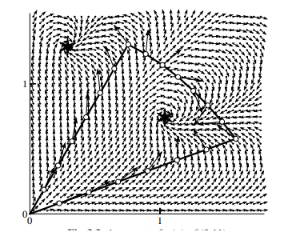
\includegraphics[width=0.5\linewidth]{images/arg_pz.png}
     \caption{Argument $p(z)$}
    Mỗi mũi tên tại điểm $z$ biểu diễn hướng của $\arg p(z)$ trên mặt phẳng phức; hai điểm được đánh dấu là các nghiệm của $p(z)$ (nguồn/đích của trường vector, tương ứng với điểm mà $\arg p(z)$ quay trọn một vòng xung quanh). Đường viền tam giác minh hoạ biên của quạt $S_j$ được xét trong chứng minh: cạnh đáy là tia $\arg z = 0$ (trục thực dương), hai cạnh còn lại là các tia biên $\arg z = 2\pi(j\mp \tfrac12)/k$. Có thể quan sát trực tiếp trên hình rằng nghiệm duy nhất của $p(z)$ nằm trong quạt $S_1$ nằm khá gần đĩa cấm $\{|z-1|\le 1\}$.
 \end{figure}
\noindent\textbf{Chặn trên cho phần dao động $I_1$}
Bước tiếp theo là chứng minh rằng nghiệm duy nhất nói trên, với $k$ đủ
lớn, thực sự rơi vào bên trong đĩa cấm $\{|z-1|\le 1\}$. Ta tách tích phân
\eqref{eq:bdf-p-integral} thành hai phần,
\[
p(z) = I_1 - I_2, \qquad
I_1 = \int_0^{r} \varphi(s)\,ds - e^{ik\theta}\int_0^{1} s^{k}\varphi(s)\,ds,
\qquad
I_2 = e^{ik\theta}\int_1^{r} s^{k}\varphi(s)\,ds,
\]
tức tách phần ứng với $s\le 1$ (dao động, bị chặn) khỏi phần ứng với
$s>1$ (tăng theo lũy thừa $s^k$).
 
Với hàm trọng $\varphi(s)$, ta có chặn
\[
|\varphi(s)| \le B(\theta), \qquad
B(\theta) = \begin{cases} |\sin\theta|^{-1}, & 0 < \theta \le \pi/2 \text{ hoặc } 3\pi/2 \le \theta < 2\pi,\\[2pt] 1, & \text{còn lại}. \end{cases}
\]
Ước lượng trực tiếp các tích phân trong $I_1$ (dùng chặn trên của
$\varphi$ và bất đẳng thức tam giác) dẫn tới
\begin{equation}
|I_1| \;\le\; \Bigl(r + \frac{1}{k+1}\Bigr) B(\theta)\;<\; r\,B(\theta)\,\frac{k+2}{k+1}, \qquad (r>1).\tag{3.2}\label{eq:3.2}
\end{equation}
 
\noindent\textbf{Chặn dưới cho phần tăng $I_2$}
 
Vì $s^{k}$ luôn dương trên đoạn lấy tích phân, ta có thể viết $I_2$ dưới
dạng
\[
I_2 = e^{ik\theta}\,\Phi \int_1^{r} s^{k}\,ds,
\qquad \Phi \in \text{bao lồi của } \{\varphi(s) : 1\le s\le r\}.
\]

Mọi phần tử của bao lồi này có thể viết dưới dạng
\[
\Phi = \alpha\,\varphi(s_1) + (1-\alpha)\,\varphi(s_2)
= \frac{\varphi(s_1)\,\varphi(s_2)}{\varphi(\hat s)},
\qquad 0\le\alpha\le 1,\ 1\le s_1,s_2\le r,
\]
với $\hat s = \alpha s_1 + (1-\alpha)s_2$. Do $|\varphi(s)|$ giảm đơn điệu theo $s$ khi $s\ge 1$, ta suy ra $|\Phi| \ge |\varphi(r)|$. Kết hợp với
$$\int_1^r s^k\,ds = (r^{k+1}-1)/(k+1)$$
ta được
\begin{equation}
|I_2| \;\ge\; \frac{r^{k+1}-1}{2r(k+1)} \;>\; \frac{r\bigl(r^{k-1}-1\bigr)}{2k+2}, \qquad (r>1).
\label{eq:bdf-I2-bound}
\end{equation}
 
\noindent\textbf{Kết hợp hai chặn và kết luận}
 
So sánh \eqref{eq:3.2} và \eqref{eq:3.3}, ta thấy rằng nếu
\begin{equation*}
r \;\ge\; R(\theta) := \Bigl( (2k+4)\,B(\theta) + 1 \Bigr)^{1/(k-1)}, \tag{3.3}\label{eq:3.3}
\end{equation*}
thì $|I_2| > |I_1|$, và do đó $p(z) = I_1 - I_2 \ne 0$ tại điểm
$z=re^{i\theta}$ đó. Nói cách khác, đường cong $r = R(\theta)$ cắt ra khỏi mỗi quạt $S_j$ một phần mà bên trong nó \emph{chắc chắn không} có nghiệm nào của $p(z)$ — phần còn lại giữa đường cong này và đĩa cấm $\{|z-1|\le 1\}$ chính là nơi duy nhất nghiệm của $p(z)$ trong quạt đó có thể có.
 
Với $k=12$, phần diện tích còn lại này đã đủ nhỏ để đảm bảo nghiệm duy
nhất trong quạt $S_1$ ($j\ne 0$) buộc phải nằm bên trong đĩa
$\{|z-1|\le 1\}$ — tức công thức BDF không ổn định tại $k=12$. Vì
$R(\theta)$ giảm đơn điệu theo $k$ với $\theta$ cố định (và điều tương tự đúng cho $R(\pi/k)$), điều này còn đúng cho mọi $k\ge 12$.
 
Với các giá trị trung gian $6 < k < 12$, tính không ổn định được xác nhận bằng tính toán số trực tiếp các nghiệm của $p(z)$.

\begin{figure}[H]
    \centering
    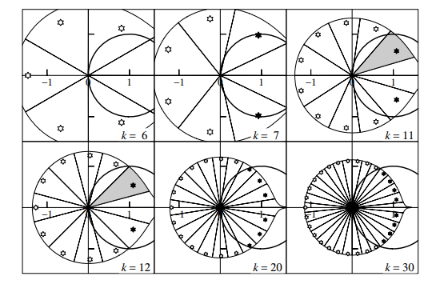
\includegraphics[width=0.85\textwidth]{images/root_pz.png}
    \caption{Phân bố các nghiệm của đa thức  $p_k(z)=\sum_{j=1}^{k}\frac{z^j}{j}$ trên mặt phẳng phức đối với một số giá trị của $k$. Đường tròn có tâm tại $(1,0)$ và bán kính $1$ biểu diễn miền $\{z:|z-1|<1\}$.
    Khi $k\le6$, mọi nghiệm đều nằm ngoài miền này; từ $k=7$ trở đi bắt đầu xuất hiện nghiệm nằm trong đĩa $|z-1|<1$, do đó điều kiện nghiệm của phương pháp BDF không còn được thỏa mãn.}
    \label{fig:roots-pk}
\end{figure}
Hình~\ref{fig:roots-pk} minh họa trực quan sự thay đổi vị trí các nghiệm của đa thức $p_k(z)$ khi số bước $k$ tăng. Có thể thấy rằng đối với $k=6$, toàn bộ các nghiệm vẫn nằm ngoài đĩa $|z-1|<1$, trong khi từ $k=7$ đã xuất hiện nghiệm đi vào miền này. Theo phép biến đổi Möbius, điều đó tương đương với việc đa thức đặc trưng của phương pháp BDF xuất hiện nghiệm có môđun lớn hơn $1$, làm vi phạm điều kiện 0-ổn định. Quan sát này phù hợp với kết quả của Định lý Dahlquist rằng họ phương pháp BDF chỉ 0-ổn định đối với $k\le6$.

Bảng tổng hợp kết quả về tính $0$-ổn định của các phương pháp BDF như sau.

\begin{table}[H]
\centering
\caption{Tính $0$-ổn định của các phương pháp BDF}
\label{tab:bdf-zero-stability}
\begin{tabular}{cc}
\hline
Bậc $k$ & Tính $0$-ổn định\\
\hline
$1\le k\le6$ & Có\\
$k\ge7$ & Không\\
\hline
\end{tabular}
\end{table}


\subsubsection{Kiểm chứng bằng số ranh giới $k \leq 6$}

Kết luận trên có thể được kiểm chứng trực tiếp bằng cách giải số phương trình
$\rho(z)=0$ cho từng giá trị $k$ và so sánh môđun lớn nhất trong các nghiệm với $1$.
Bảng~\ref{tab:bdf-stability} được sinh tự động từ mã nguồn đi kèm: với mỗi $k$, hệ số
của phương pháp BDF được dựng lại từ khai triển sai phân lùi
$\sum_{j=1}^{k}\frac{1}{j}\nabla^{j}Y_{n+k}=hf_{n+k}$, sau đó nghiệm của đa thức đặc
trưng thứ nhất được tính bằng phương pháp số.

\input{Sections/generated/bdf_stability}

Có thể thấy với mọi $k\le 6$, môđun lớn nhất đúng bằng $1$ và nghiệm đạt giá trị này
chính là nghiệm chính $z=1$ (nghiệm đơn), nên điều kiện nghiệm được thỏa mãn. Từ $k=7$,
môđun lớn nhất vượt ngưỡng ($1.0222$ khi $k=7$ và $1.1839$ khi $k=8$), phá vỡ điều kiện
nghiệm. Ranh giới $k\le 6$ vì vậy không phải là một quy ước được áp đặt, mà xuất hiện
như hệ quả trực tiếp từ vị trí nghiệm của đa thức đặc trưng.

\begin{figure}[H]
    \centering
    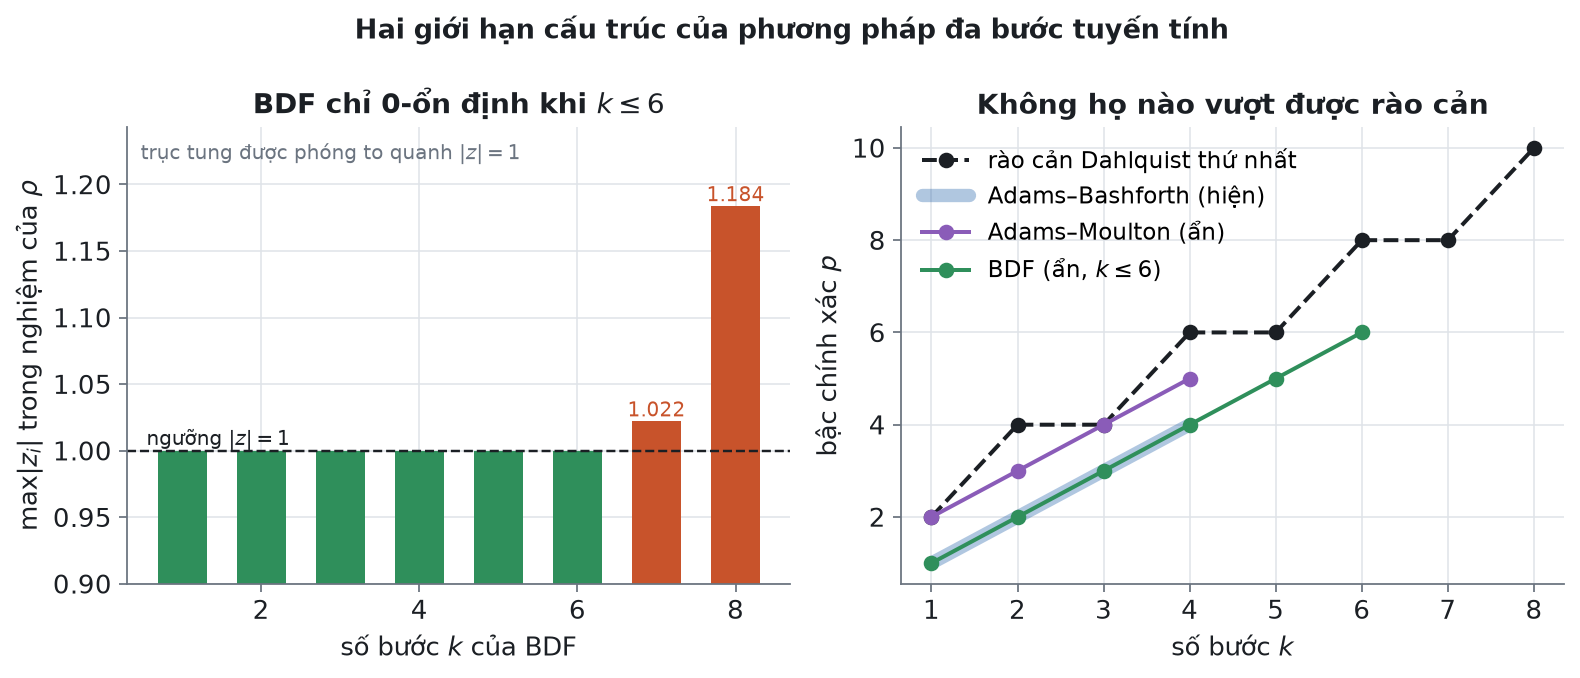
\includegraphics[width=\textwidth]{figures/fig06_dahlquist_barrier.png}
    \caption{Trái: môđun lớn nhất trong các nghiệm của $\rho(z)$ đối với họ BDF, trục
    tung được phóng to quanh ngưỡng $|z|=1$; các cột đỏ ($k=7,8$) vượt ngưỡng.
    Phải: bậc chính xác của ba họ phương pháp so với rào cản Dahlquist thứ nhất
    ($p\le k+2$ khi $k$ chẵn, $p\le k+1$ khi $k$ lẻ). Đường Adams--Bashforth được vẽ
    dày và mờ vì trùng hoàn toàn với đường BDF: cả hai đều có $p=k$.}
    \label{fig:dahlquist-barrier}
\end{figure}

\subsubsection{Miền ổn định tuyệt đối và bài toán cứng}

Tính $0$-ổn định là điều kiện khi $h\to 0$; trong tính toán thực tế, câu hỏi quan trọng
không kém là với một bước lưới $h$ \emph{cố định}, phương pháp chịu được những giá trị
$h\lambda$ nào. Miền ổn định tuyệt đối được xác định qua quỹ tích biên: ảnh của đường
tròn đơn vị dưới ánh xạ $z\mapsto \rho(z)/\sigma(z)$.

\begin{figure}[H]
    \centering
    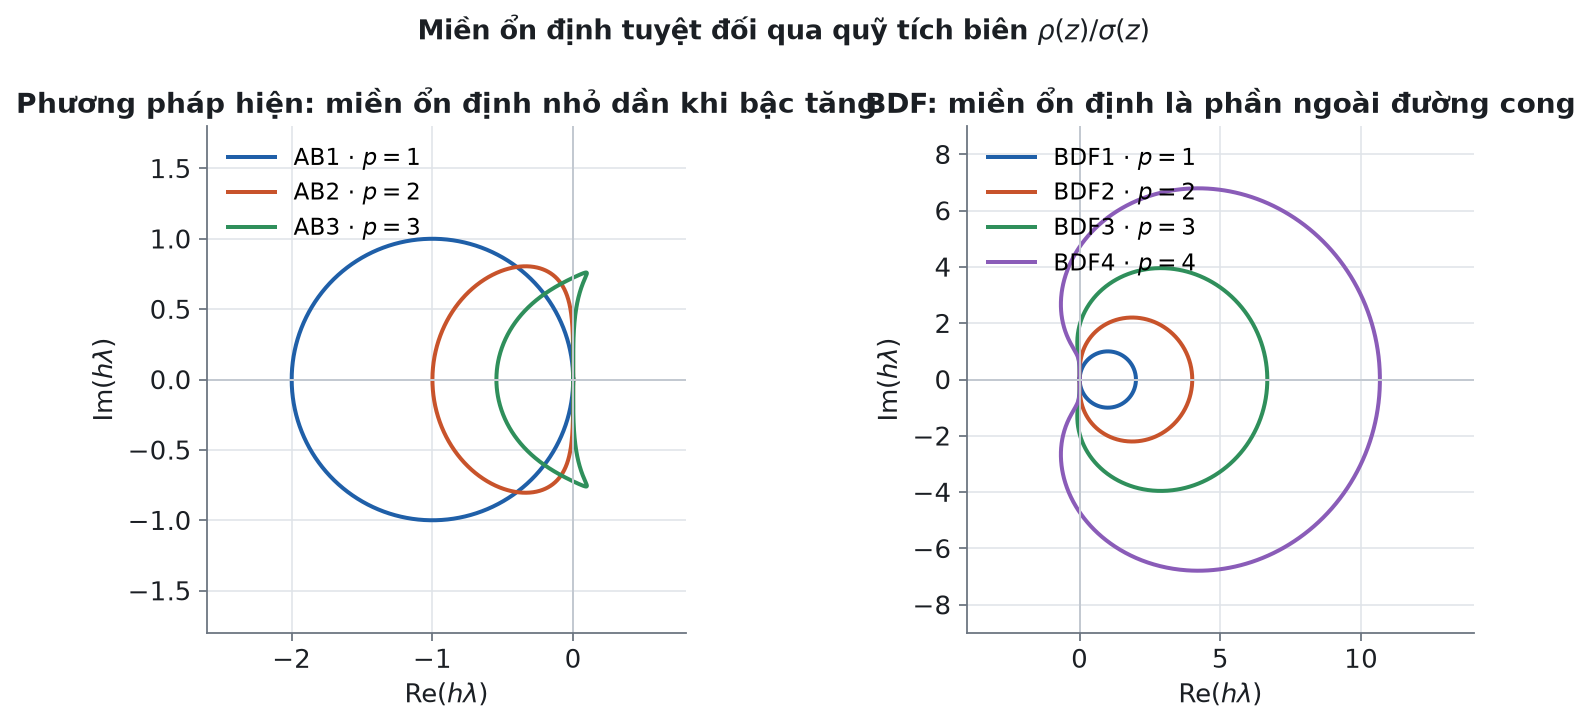
\includegraphics[width=\textwidth]{figures/fig05_stability_regions.png}
    \caption{Biên miền ổn định tuyệt đối. Với họ Adams--Bashforth (trái), miền ổn định
    nằm \emph{bên trong} đường cong và co lại nhanh khi bậc tăng: khoảng ổn định trên
    trục thực âm giảm từ $(-2,0)$ với AB1 xuống $(-6/11,0)\approx(-0.546,0)$ với AB3.
    Với họ BDF (phải), miền ổn định là phần \emph{bên ngoài} đường cong và chứa toàn bộ
    trục thực âm, nên bước lưới không bị ràng buộc bởi thành phần tắt dần nhanh.}
    \label{fig:stability-regions}
\end{figure}

Đây chính là lý do họ BDF được ưa dùng cho các bài toán cứng (stiff). Với bài toán
$y'=-1000\,(y-\cos t)-\sin t$, $y(0)=1$ và bước lưới $h=0.05$, ta có $h\lambda=-50$ nằm
ngoài miền ổn định của AB2 nên nghiệm số nổ tung, trong khi BDF2 vẫn cho sai số nhỏ hơn
$10^{-2}$. Cần nhấn mạnh rằng hai khái niệm là độc lập: AB2 vẫn $0$-ổn định và vẫn hội
tụ khi $h\to 0$, nhưng ở một bước lưới cụ thể thì hoàn toàn không dùng được.

\newpage
\section{Chương 4: Minh họa bằng phương pháp số}
\subsection{Ví dụ 1}
Định lý Dahlquist khẳng định rằng một phương pháp đa bước tuyến tính hội tụ khi và chỉ khi nó vừa nhất quán, vừa 0-ổn định. Để thấy rõ vai trò không thể thiếu của điều kiện 0-ổn định - tức là để chỉ ra rằng tính nhất quán, dù đạt bậc chính xác cao, vẫn không đủ để đảm bảo hội tụ nếu điều kiện nghiệm bị vi phạm. 

\begin{vidu}{Ví dụ 1}
    Xét phương pháp đa bước tuyến tính hai bước
    \begin{equation*}
        Y_{n+2}+4Y_{n+1}-5Y_n=h\left(4f_{n+1}+2f_n\right),
    \end{equation*}
    trong đó $f_n=f(t_n,Y_n)$. Gọi phương pháp này là \emph{phương pháp A}.
\end{vidu}



\subsubsection*{Kiểm tra tính nhất quán}
Một phương pháp đa bước tuyến tính được gọi là nhất quán nếu nó thỏa hai điều kiện sau:
$\rho(1) = 0$ và $\rho'(1) = \sigma(1)$. 
Thay $z = 1$ vào $\rho(z)$:
$$\rho(1) = 1^2 + 4(1) - 5 = 1 + 4 - 5 = 0$$
$$\rho'(z) = 2z + 4 \implies \rho'(1) = 2(1) + 4 = 6$$

Tính giá trị của $\sigma(1)$:
$$\sigma(1) = 4(1) + 2 = 6$$

Ta thấy $\rho(1) = 0$ và $\rho'(1) = \sigma(1) = 6$. Vậy phương pháp A nhất quán. 

\subsubsection*{Kiểm tra điều kiện nghiệm}

Đa thức đặc trưng thứ nhất:
\[
\rho(z)=z^2+4z-5=(z-1)(z+5)=0
\]
\[
\Leftrightarrow z_1=1,\qquad z_2=-5.
\]

Theo điều kiện nghiệm, mọi nghiệm của $\rho(z)$ phải có môđun không vượt quá $1$, đồng thời các nghiệm nằm trên đường tròn đơn vị phải là nghiệm đơn. Tuy nhiên,
\[
|z_2|=5>1,
\]
nên phương pháp A không thỏa điều kiện nghiệm. Theo Định lý Dahlquist, phương pháp không 0-ổn định.

\subsubsection*{Mô phỏng nghiệm số}

Nhằm minh họa cho các phân tích lý thuyết, phương pháp A được áp dụng để giải bài toán giá trị ban đầu:
\[
y'(t) = -y(t),\qquad y(0) = 1.
\]
Nghiệm chính xác của bài toán là $y(t) = e^{-t}$.

\begin{lstlisting}[style=MatlabStyle,caption={Mã MATLAB cho phương pháp A.},label={lst:methodA}]
clear; clc; close;

% ---- Thiet lap bai toan ----
f      = @(t, y) -y;          % ve phai phuong trinh vi phan
y_exact = @(t) exp(-t);       % nghiem chinh xac
t0 = 0;
T  = 6;                        % thoi diem cuoi
h  = 0.1;                      % buoc luoi

N = round((T - t0) / h);
t = t0 + (0:N) * h;

% ---- Khoi tao (lay tu nghiem giai tich, loai bo sai so khoi tao) ----
y = zeros(1, N + 1);
y(1) = y_exact(t(1));   % y0
y(2) = y_exact(t(2));   % y1

% ---- Vong lap Phuong phap A (hien) ----
for n = 1:(N - 1)
    fn1 = f(t(n+1), y(n+1));   % f_{n+1}
    fn  = f(t(n),   y(n));     % f_n
    y(n+2) = -4*y(n+1) + 5*y(n) + h * (4*fn1 + 2*fn);
end

% ---- Nghiem chinh xac va sai so ----
yex = y_exact(t);
err = abs(y - yex);

% ---- In bang ket qua tai mot so moc thoi gian ----
moc = [0.0, 0.5, 1.0, 2.0, 4.0, 6.0];
fprintf('%8s %18s %18s %14s\n', 't', 'Nghiem chinh xac', 'Phuong phap A', 'Sai so |y-yex|');
for k = 1:length(moc)
    [~, idx] = min(abs(t - moc(k)));
    fprintf('%8.1f %18.6e %18.6e %14.3e\n', t(idx), yex(idx), y(idx), err(idx));
end


thresh = 1;
symlog = @(x) sign(x) .* log10(1 + abs(x) / thresh);

% ---- Do thi ----

% Thang symlog
figure(1);
plot(t, symlog(yex), 'k-', 'LineWidth', 1.5); hold on;
plot(t, symlog(y),   'r--', 'LineWidth', 1.2);
legend('Nghiem chinh xac', 'Phuong phap A', 'Location', 'best');
xlabel('t'); ylabel('symlog( y(t) )');
title('So sanh nghiem: Phuong phap A vs nghiem chinh xac (truc y thang symlog)');
grid on;

% Ve lai nhan truc tung theo gia tri that
yt = get(gca, 'YTick');
yticklabels_real = arrayfun(@(v) sprintf('%.0e', sign(v)*(10^abs(v)-1)*thresh), yt, 'UniformOutput', false);
set(gca, 'YTickLabel', yticklabels_real);

% Thang binh thuong
figure(2);
subplot(3,1,2);
plot(t, yex, 'k-', 'LineWidth', 1.5); hold on;
plot(t, y,   'r--', 'LineWidth', 1.2);
legend('Nghiem chinh xac', 'Phuong phap A', 'Location', 'best');
xlabel('t'); ylabel('y(t)');
title('So sanh nghiem: Phuong phap A va nghiem chinh xac');
grid on;

% Thang log cho sai so
figure(3);
semilogy(t, err, 'b-', 'LineWidth', 1.2);
xlabel('t'); ylabel('Sai so tuyet doi |y - y_{exact}|');
title('Sai so tuyet doi theo thoi gian (thang log)');
grid on;
\end{lstlisting}
\begin{figure}[H]
    \centering
    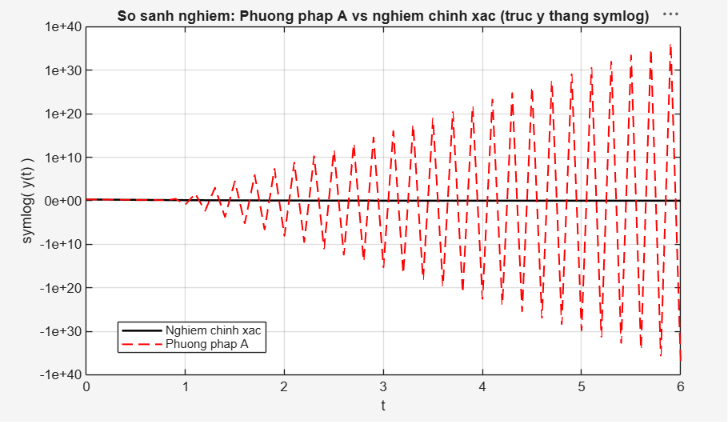
\includegraphics[width=\textwidth]{images/vd1_1.png}
    \caption{So sánh nghiệm số của phương pháp A và nghiệm chính xác. Trục tung sử dụng thang đo \texttt{symlog} (symmetric log).}
\end{figure}

\begin{figure}[H]
    \centering
    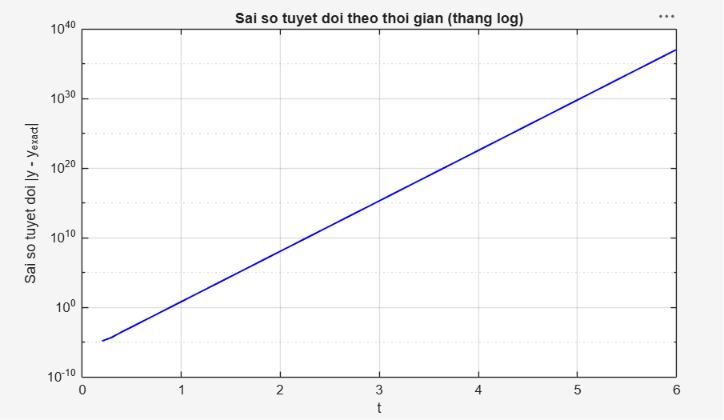
\includegraphics[width=\textwidth]{images/vd1_3.png}
    \caption{Đồ thị sai số của phương pháp A}
\end{figure}
\begin{table}[H]
\centering
\caption{So sánh nghiệm chính xác, nghiệm số của phương pháp A và sai số tuyệt đối tại một số thời điểm.}
\renewcommand{\arraystretch}{1.2}
\begin{tabular}{cccc}
\toprule
$t$ & $y_n$ & $Y_n$ & $E_n$\\
\midrule
0.0 & $1.000000\times10^{0}$  & $1.000000\times10^{0}$  & $0$\\
0.5 & $6.065307\times10^{-1}$ & $6.081996\times10^{-1}$ & $1.668921\times10^{-3}$\\
1.0 & $3.678794\times10^{-1}$ & $-6.677259\times10^{0}$ & $7.045138\times10^{0}$\\
2.0 & $1.353353\times10^{-1}$ & $-1.243391\times10^{8}$ & $1.243391\times10^{8}$\\
4.0 & $1.831564\times10^{-2}$ & $-3.872979\times10^{22}$ & $3.872979\times10^{22}$\\
6.0 & $2.478752\times10^{-3}$ & $-1.206376\times10^{37}$ & $1.206376\times10^{37}$\\
\bottomrule
\end{tabular}
\end{table}

\subsubsection*{Phân tích kết quả}

Kết quả thực nghiệm cho thấy trong những bước tính đầu tiên, nghiệm số của phương pháp A còn khá gần với nghiệm chính xác. Tuy nhiên, khi số bước lưới tăng lên, sai số bắt đầu tăng rất nhanh và nghiệm số nhanh chóng phân kỳ khỏi nghiệm đúng. Từ Bảng trên có thể thấy tại $t=1$, sai số đã đạt khoảng $7.05$, trong khi tại $t=6$ sai số lên tới khoảng $1.21\times10^{37}$.

Hiện tượng phân kỳ của phương pháp A có thể được giải thích trực tiếp thông qua nghiệm của phương trình sai phân tương ứng. Đối với bài toán
\[
y'(t)=-y(t),\qquad y(0)=1,
\]
ta có
\[
f_n=-Y_n.
\]

Thay vào công thức của phương pháp A thu được
\[
Y_{n+2}+4(1-h)Y_{n+1}-(5+2h)Y_n=0.
\]

Phương trình đặc trưng tương ứng là
\[
\lambda^2+4(1-h)\lambda-(5+2h)=0.
\]

Khi $h$ đủ nhỏ, hai nghiệm của phương trình đặc trưng có dạng
\[
\lambda_1=1+O(h),\qquad
\lambda_2=-5+O(h).
\]

Do đó nghiệm tổng quát của phương trình sai phân được biểu diễn dưới dạng
\[
Y_n=C_1\lambda_1^n+C_2\lambda_2^n,
\]
trong đó các hằng số $C_1,C_2$ phụ thuộc vào điều kiện ban đầu. Vì
\[
|\lambda_2|\approx5>1,
\]
thành phần $C_2\lambda_2^n$ được khuếch đại khoảng $5$ lần sau mỗi bước lặp. Mặc dù sai số ban đầu có thể rất nhỏ, thành phần này vẫn tăng theo cấp số nhân và nhanh chóng lấn át nghiệm thực của bài toán. Chính cơ chế khuếch đại này làm cho nghiệm số phân kỳ mặc dù phương pháp vẫn thỏa điều kiện nhất quán.

\subsection{Ví dụ 2}
\begin{vidu}{Ví dụ 2}
    Xét phương pháp đa bước tuyến tính hai bước, được gọi là \emph{phương pháp B}
    \begin{equation*}
        Y_{n+2}-4Y_{n+1}+3Y_n=-2h\,f_{n+2}.
    \end{equation*}
\end{vidu}


\subsubsection*{Kiểm tra tính nhất quán}

Một phương pháp đa bước tuyến tính được gọi là nhất quán nếu nó thỏa hai điều kiện sau: $\rho(1) = 0$ và $\rho'(1) = \sigma(1)$. Thay $z = 1$ vào $\rho(z)$:

$$ \rho(1) = 1^2 - 4(1) + 3 = 1 - 4 + 3 = 0 $$

$$ \rho'(z) = 2z - 4 \implies \rho'(1) = 2(1) - 4 = -2 $$

Tính giá trị của $\sigma(1)$:

$$ \sigma(1) = -2(1)^2 = -2 $$

Ta thấy $\rho(1) = 0$ và $\rho'(1) = \sigma(1) = -2$. Vậy phương pháp nhất quán.

\vspace{0.5cm}
\subsubsection*{Kiểm tra điều kiện nghiệm}

Đa thức đặc trưng thứ nhất:

\[
    \rho(z) = z^2 - 4z + 3 = (z - 1)(z - 3) = 0
\]  

\[
    z_1 = 1, \qquad z_2 = 3
\] 

Theo điều kiện nghiệm, mọi nghiệm của $\rho(z)$ phải có môđun không vượt quá 1, đồng thời các nghiệm nằm trên đường tròn đơn vị phải là nghiệm đơn. Tuy nhiên,
\[
|z_2| = 3 > 1, 
\]
nên phương pháp không thỏa điều kiện nghiệm. Theo Định lý Dahlquist, phương pháp không hội tụ.

\subsubsection*{Mô phỏng nghiệm số}

Nhằm minh họa cho các phân tích lý thuyết, phương pháp B được áp dụng để giải bài toán giá trị ban đầu:
\[
y'(t) = -y(t),\qquad y(0) = 1.
\]

Nghiệm chính xác của bài toán là $y(t) = e^{-t}$.

\begin{lstlisting}[style=MatlabStyle,caption={Mã MATLAB cho phương pháp B.},label={lst:methodB}]
clear; clc; close all;

% Thiet lap bai toan
f       = @(t, y) -y;          
y_exact = @(t) exp(-t);       
t0 = 0;
T  = 6;                       
h  = 0.1;                     
N  = round((T - t0) / h);
t  = t0 + (0:N) * h;

% Khoi tao
y = zeros(1, N + 1);
y(1) = y_exact(t(1));   % y0
y(2) = y_exact(t(2));   % y1

% Phuong phap B
for n = 1:(N - 1)
    y(n+2) = (4*y(n+1) - 3*y(n)) / (1 - 2*h);
end

% Nghiem chinh xac va sai so
yex = y_exact(t);
err = abs(y - yex);

% ---- In bang ket qua tai mot so moc thoi gian ----
moc = [0.0, 0.5, 1.0, 2.0, 4.0, 6.0];
fprintf('%8s %18s %18s %14s\n', 't', 'Nghiem chinh xac', 'Phuong phap', 'Sai so');
for k = 1:length(moc)
    [~, idx] = min(abs(t - moc(k)));
    fprintf('%8.1f %18.6e %18.6e %14.3e\n', t(idx), yex(idx), y(idx), err(idx));
end

thresh = 1;
symlog = @(x) sign(x) .* log10(1 + abs(x) / thresh);

% ---- Do thi ----

% Hinh 1: Thang symlog
figure(1);
plot(t, symlog(yex), 'k-', 'LineWidth', 1.5); hold on;
plot(t, symlog(y),   'r--', 'LineWidth', 1.2);
legend('Nghiem chinh xac', 'Phuong phap B', 'Location', 'best');
xlabel('t'); ylabel('symlog( y(t) )');
title('Hinh 1: Phuong phap B vs Nghiem chinh xac (truc y thang symlog)');
grid on;

% Ve lai nhan truc tung theo gia tri that (chi de doc so, khong anh huong tinh toan)
yt = get(gca, 'YTick');
yticklabels_real = arrayfun(@(v) sprintf('%.0e', sign(v)*(10^abs(v)-1)*thresh), yt, 'UniformOutput', false);
set(gca, 'YTickLabel', yticklabels_real);

% Hinh 2: Thang binh thuong
figure(2);
plot(t, yex, 'k-', 'LineWidth', 1.5); hold on;
plot(t, y,   'r--', 'LineWidth', 1.2);
legend('Nghiem chinh xac', 'Phuong phap B', 'Location', 'best');
xlabel('t'); ylabel('y(t)');
title('Hinh 2: Phuong phap B va Nghiem chinh xac');
grid on;

% Hinh 3: Thang log cho sai so
figure(3);
semilogy(t, err, 'b-', 'LineWidth', 1.2);
xlabel('t'); ylabel('Sai so tuyet doi |y - y_{exact}|');
title('Hinh 3: Sai so tuyet doi theo thoi gian (thang log)');
grid on;
\end{lstlisting}
\begin{figure}[H]
    \centering
    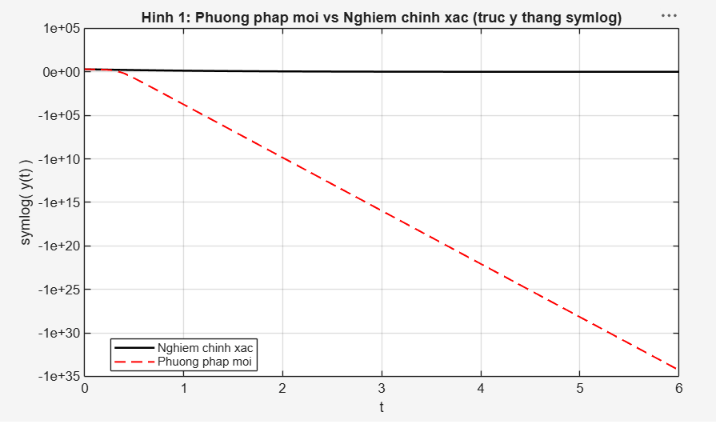
\includegraphics[width=\textwidth]{images/vd2_1.png}
    \caption{So sánh nghiệm số của phương pháp B và nghiệm chính xác. Trục tung sử dụng thang đo \texttt{symlog} (symmetric log).}
\end{figure}

\begin{figure}[H]
    \centering
    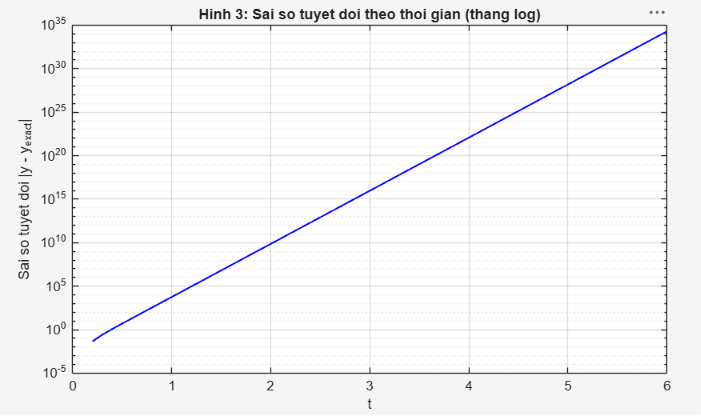
\includegraphics[width=\textwidth]{images/vd2_3.png}
    \caption{Đồ thị sai số của phương pháp B}
\end{figure}
\begin{table}[H]
\centering
\caption{So sánh nghiệm chính xác, nghiệm số của phương pháp B và sai số tuyệt đối tại một số thời điểm.}
\renewcommand{\arraystretch}{1.2}
\begin{tabular}{cccc}
\toprule
$t$ & $y_n$ & $Y_n$ & $E_n$\\
\midrule
0.0 & 1.000000e+00 & \phantom{-}1.000000e+00 & 0 \\
0.5 & 6.065307e-01 & -4.362861e+00 & 4.969e+00 \\
1.0 & 3.678794e-01 & -5.683881e+03 & 5.684e+03 \\
2.0 & 1.353353e-01 & -7.286041e+09 & 7.286e+09 \\
4.0 & 1.831564e-02 & -1.197068e+22 & 1.197e+22 \\
6.0 & 2.478752e-03 & -1.966737e+34 & 1.967e+34 \\
\bottomrule
\end{tabular}
\end{table}

\subsubsection*{Phân tích kết quả}

Kết quả mô phỏng cho thấy phương pháp B cũng không cho nghiệm hội tụ về nghiệm chính xác. Ngay từ những bước tính đầu tiên, sai số đã tăng nhanh và tiếp tục khuếch đại theo thời gian. Từ Bảng trên có thể thấy sai số tại $t=0.5$ đã đạt gần $5$, và đến $t=6$ đạt xấp xỉ $1.97\times10^{34}$.

Hiện tượng phân kỳ của phương pháp B cũng có thể được giải thích thông qua nghiệm của phương trình sai phân tương ứng. Đối với bài toán
\[
y'(t)=-y(t),\qquad y(0)=1,
\]
ta có
\[
f_{n+2}=-Y_{n+2}.
\]

Thay vào công thức của phương pháp B thu được
\[
(1-2h)Y_{n+2}-4Y_{n+1}+3Y_n=0.
\]

Phương trình đặc trưng tương ứng là
\[
(1-2h)\lambda^2-4\lambda+3=0.
\]

Khi $h$ đủ nhỏ, hai nghiệm của phương trình đặc trưng có dạng
\[
\lambda_1=1+O(h),\qquad
\lambda_2=3+O(h).
\]

Do đó nghiệm tổng quát của phương trình sai phân được biểu diễn dưới dạng
\[
Y_n=C_1\lambda_1^n+C_2\lambda_2^n,
\]
trong đó các hằng số $C_1,C_2$ phụ thuộc vào điều kiện ban đầu. Vì
\[
|\lambda_2|\approx3>1,
\]
thành phần $C_2\lambda_2^n$ được khuếch đại xấp xỉ $3$ lần sau mỗi bước lặp. Mặc dù sai số ban đầu có thể rất nhỏ, thành phần này vẫn tăng theo cấp số nhân và nhanh chóng lấn át nghiệm thực của bài toán. Chính cơ chế khuếch đại này làm cho nghiệm số phân kỳ mặc dù phương pháp vẫn thỏa điều kiện nhất quán.

\subsubsection*{Tóm tắt}
Hai ví dụ thực nghiệm trong chương này đã minh họa trực quan các kết quả của định lý Dashquist. Ví dụ 1 khảo sát một phương pháp đa bước tuyến tính hiện, trong khi Ví dụ 2 khảo sát một phương pháp đa bước tuyến tính ẩn. Mặc dù cả hai phương pháp đều thỏa điều kiện nhất quán, chúng đều vi phạm điều kiện nghiệm. Kết quả là sai số không bị triệt tiêu mà ngược lại còn được khuếch đại sau mỗi bước lặp, khiến nghiệm số nhanh chóng phân kỳ khỏi nghiệm chính xác.

Các bảng số liệu và đồ thị MATLAB đều cho thấy sai số tăng rất nhanh theo thời gian, hoàn toàn phù hợp với phân tích lý thuyết dựa trên điều kiện 0-ổn định. Điều này xác nhận rằng tính nhất quán chỉ là điều kiện cần, còn tính 0-ổn định mới là điều kiện quyết định để đảm bảo hội tụ của phương pháp đa bước tuyến tính.

Qua các ví dụ trên có thể rút ra rằng việc lựa chọn một phương pháp số không chỉ dựa trên bậc chính xác hay việc phương pháp là hiện hoặc ẩn, mà quan trọng hơn là phải kiểm tra điều kiện nghiệm của đa thức đặc trưng. Đây cũng chính là nội dung cốt lõi của Định lý hội tụ Dahlquist và cũng là cơ sở lý thuyết cho việc xây dựng các phương pháp ổn định trong thực tế.
\newpage

\renewcommand{\refname}{Tài liệu tham khảo}
\begin{thebibliography}{3}

\bibitem{Atkinson2009}
K. Atkinson, W. Han, and D. Stewart,
\textit{Numerical Solution of Ordinary Differential Equations},
John Wiley \& Sons, 2009.

\bibitem{Hairer1993}
E. Hairer, S. P. N{\o}rsett, and G. Wanner,
\textit{Solving Ordinary Differential Equations I: Nonstiff Problems},
2nd ed., Springer, 1993.

\bibitem{Suli2022}
E. S\"uli,
\textit{Numerical Solution of Ordinary Differential Equations},
Lecture Notes, University of Oxford, 2022.

\end{thebibliography}
\end{document}